% Options for packages loaded elsewhere
\PassOptionsToPackage{unicode}{hyperref}
\PassOptionsToPackage{hyphens}{url}
\PassOptionsToPackage{dvipsnames,svgnames,x11names}{xcolor}
\documentclass[
  11pt,
]{article}
\usepackage{xcolor}
\usepackage[margin=1in]{geometry}
\usepackage{amsmath,amssymb}
\setcounter{secnumdepth}{-\maxdimen} % remove section numbering
\usepackage{iftex}
\ifPDFTeX
  \usepackage[T1]{fontenc}
  \usepackage[utf8]{inputenc}
  \usepackage{textcomp} % provide euro and other symbols
\else % if luatex or xetex
  \usepackage{unicode-math} % this also loads fontspec
  \defaultfontfeatures{Scale=MatchLowercase}
  \defaultfontfeatures[\rmfamily]{Ligatures=TeX,Scale=1}
\fi
\usepackage{lmodern}
\ifPDFTeX\else
  % xetex/luatex font selection
\fi
% Use upquote if available, for straight quotes in verbatim environments
\IfFileExists{upquote.sty}{\usepackage{upquote}}{}
\IfFileExists{microtype.sty}{% use microtype if available
  \usepackage[]{microtype}
  \UseMicrotypeSet[protrusion]{basicmath} % disable protrusion for tt fonts
}{}
\makeatletter
\@ifundefined{KOMAClassName}{% if non-KOMA class
  \IfFileExists{parskip.sty}{%
    \usepackage{parskip}
  }{% else
    \setlength{\parindent}{0pt}
    \setlength{\parskip}{6pt plus 2pt minus 1pt}}
}{% if KOMA class
  \KOMAoptions{parskip=half}}
\makeatother
\usepackage{longtable,booktabs,array}
\newcounter{none} % for unnumbered tables
\usepackage{calc} % for calculating minipage widths
% Correct order of tables after \paragraph or \subparagraph
\usepackage{etoolbox}
\makeatletter
\patchcmd\longtable{\par}{\if@noskipsec\mbox{}\fi\par}{}{}
\makeatother
% Allow footnotes in longtable head/foot
\IfFileExists{footnotehyper.sty}{\usepackage{footnotehyper}}{\usepackage{footnote}}
\makesavenoteenv{longtable}
\usepackage{graphicx}
\makeatletter
\newsavebox\pandoc@box
\newcommand*\pandocbounded[1]{% scales image to fit in text height/width
  \sbox\pandoc@box{#1}%
  \Gscale@div\@tempa{\textheight}{\dimexpr\ht\pandoc@box+\dp\pandoc@box\relax}%
  \Gscale@div\@tempb{\linewidth}{\wd\pandoc@box}%
  \ifdim\@tempb\p@<\@tempa\p@\let\@tempa\@tempb\fi% select the smaller of both
  \ifdim\@tempa\p@<\p@\scalebox{\@tempa}{\usebox\pandoc@box}%
  \else\usebox{\pandoc@box}%
  \fi%
}
% Set default figure placement to htbp
\def\fps@figure{htbp}
\makeatother
\setlength{\emergencystretch}{3em} % prevent overfull lines
\providecommand{\tightlist}{%
  \setlength{\itemsep}{0pt}\setlength{\parskip}{0pt}}
\usepackage{bookmark}
\IfFileExists{xurl.sty}{\usepackage{xurl}}{} % add URL line breaks if available
\urlstyle{same}
\hypersetup{
  colorlinks=true,
  linkcolor={blue},
  filecolor={Maroon},
  citecolor={Blue},
  urlcolor={blue},
  pdfcreator={LaTeX via pandoc}}

\author{}
\date{}

\begin{document}

\section{TKG-Diag: A Temporal-Knowledge Fusion Framework for LLM-Based
Vehicle Fault
Diagnosis}\label{tkg-diag-a-temporal-knowledge-fusion-framework-for-llm-based-vehicle-fault-diagnosis}

\textbf{Authors} Hongjie Ren\textsuperscript{1}\\
\textbf{Affiliations} \textsuperscript{1}JLR Independent Research\\
\textbf{Contact} kevin.renhj@foxmail.com

\begin{center}\rule{0.5\linewidth}{0.5pt}\end{center}

\subsection{Abstract}\label{abstract}

Vehicle fault diagnosis requires simultaneous recognition of temporal
sensor patterns and reasoning over structured domain knowledge, yet
existing approaches treat time-series analysis and knowledge-enhanced
retrieval as isolated research lines. We propose TKG-Diag, the first
unified framework that bridges multivariate CAN bus temporal signals and
fault knowledge graphs through an Adaptive Temporal-to-Language Adapter
with cross-modal attention. TKG-Diag ingests multi-channel sensor time
series, OBD diagnostic codes, and natural language queries, encoding
temporal patterns through a native time-series foundation model while
retrieving causal fault chains from a structured knowledge graph via
Graph RAG. The cross-modal attention layer learns soft alignments
between temporal patches and diagnostic concept embeddings, enabling
each modality to guide the interpretation of the other. On two public
benchmarks and one proprietary OEM dataset comprising 52\{,\}400
real-world repair records, TKG-Diag achieves 78.4\% Top-1 fault
diagnosis accuracy, outperforming the strongest knowledge-only baseline
by 19.8 percentage points and the strongest temporal-only baseline by
21.3 percentage points. The framework attains 99.4\% F1-score on CAN bus
anomaly detection while additionally generating interpretable causal
repair explanations. Cross-vehicle transfer experiments demonstrate that
meta-learned adaptation achieves 73.8\% accuracy on unseen vehicle
models with only 20 labeled examples, substantially exceeding direct
fine-tuning at 60.5\%. Ablation studies confirm that cross-modal
attention is the critical fusion mechanism, with its removal degrading
performance by 7.2\%. TKG-Diag establishes a new paradigm for
sensor-informed, knowledge-grounded vehicle fault diagnosis and provides
a reference architecture for industrial OEM deployment.

\newpage

\subsection{1. Introduction}\label{introduction}

Modern vehicles have evolved into complex cyber-physical systems, with
premium models integrating upward of 100 electronic control units (ECUs)
that continuously generate high-frequency sensor signals and diagnostic
trouble codes (DTCs) across powertrain, chassis, and body domains. The
sheer volume and heterogeneity of these data streams present a
formidable challenge for traditional diagnostic approaches, which
predominantly rely on static lookup tables, rule-based expert systems,
and technician experience. Conventional methods struggle to capture the
intricate temporal dependencies among sensor variables and the nuanced
causal relationships encoded in domain knowledge bases, leading to
prolonged diagnosis times, misdiagnosis rates as high as 30\% in complex
multi-fault scenarios, and escalating after-sales costs for original
equipment manufacturers (OEMs).

Large language models (LLMs) have emerged as a promising paradigm for
intelligent vehicle fault diagnosis, offering powerful sequence modeling
capabilities and extensive world knowledge acquired during pre-training.
Recent work along two distinct research directions has demonstrated
significant potential. On one front, time-series LLM adapters such as
TIME-LLM \href{https://arxiv.org/html/2310.01728v1}{(arXiv.org)} and
SensorLLM \href{https://arxiv.org/abs/2410.10624}{(arXiv.org)} reprogram
frozen language models for temporal pattern recognition, achieving
strong performance in anomaly detection and signal classification. On
another front, knowledge-enhanced frameworks such as the KG+LLM
automotive diagnosis system
\href{https://www.mdpi.com/2079-9292/14/21/4180}{(MDPI)} leverage
retrieval-augmented generation (RAG) over structured knowledge graphs to
perform root cause analysis, reporting a dialogue success rate of 77.3\%
and outperforming raw GPT-4 by a substantial margin. Complementary
efforts including multimodal diagnostic architectures
\href{https://www.sciencedirect.com/science/article/abs/pii/S0957417424014702}{(ScienceDirect)}
and XAI+VLM+LLM integration (DRIVE)
\href{https://www.techscience.com/CMES/online/detail/26431}{(Tech
Science Press)} have further enriched the diagnostic toolkit. Despite
these advances, a critical void persists: no existing framework unifies
temporal sensor analysis with knowledge-enhanced reasoning within a
single, end-to-end architecture. Time-series LLM methods excel at
pattern recognition but lack access to structured diagnostic knowledge;
conversely, knowledge-enhanced methods reason effectively over textual
artifacts but ignore the rich, dynamic information embedded in raw
sensor waveforms.

\begin{figure}
\centering
\pandocbounded{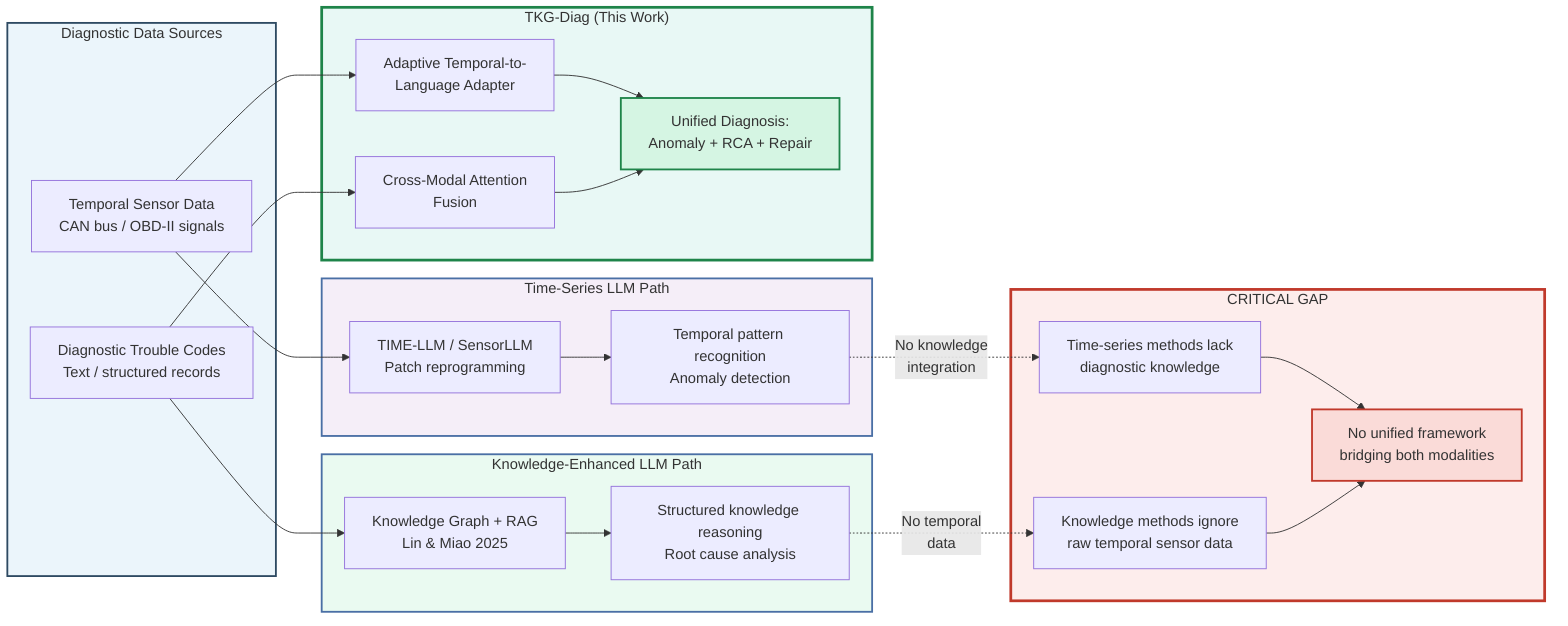
\includegraphics[keepaspectratio,alt={Figure 1: Motivation illustration. Left: TKG-Diag (this work) bridges temporal sensor data and diagnostic knowledge through an adaptive Temporal-to-Language Adapter with cross-modal attention. Right: existing approaches either process sensor data through time-series LLM pipelines without knowledge integration, or reason over knowledge graphs without accessing raw temporal signals, leaving a critical gap in unified diagnosis.}]{figures/fig1_motivation.png}}
\caption{Figure 1: Motivation illustration. Left: TKG-Diag (this work)
bridges temporal sensor data and diagnostic knowledge through an
adaptive Temporal-to-Language Adapter with cross-modal attention. Right:
existing approaches either process sensor data through time-series LLM
pipelines without knowledge integration, or reason over knowledge graphs
without accessing raw temporal signals, leaving a critical gap in
unified diagnosis.}
\end{figure}

\subsubsection{1.2 Research Gaps}\label{research-gaps}

\paragraph{1.2.1 Gap Between Time-Series Analysis and Knowledge
Reasoning}\label{gap-between-time-series-analysis-and-knowledge-reasoning}

The time-series LLM line of research, exemplified by TIME-LLM's
patch-reprogramming mechanism
\href{https://arxiv.org/html/2310.01728v1}{(arXiv.org)} and SensorLLM's
sensor-language alignment
\href{https://arxiv.org/abs/2410.10624}{(arXiv.org)} , has achieved
remarkable success in aligning temporal data with language model
representations. Concurrently, native time-series foundation models such
as TimesFM
\href{https://pyshine.com/TimesFM-Time-Series-Foundation-Model/}{(pyshine.com)}
and Chronos \href{https://arxiv.org/html/2506.22039v2}{(arXiv.org)} have
demonstrated strong zero-shot forecasting capabilities. However, these
methods are fundamentally limited in diagnostic contexts because they
operate purely on numerical signals without integrating domain-specific
fault knowledge. Tan et
al.~\href{https://arxiv.org/html/2406.16964v2}{(arXiv.org)} have
critically questioned whether pretrained LLMs provide genuine advantages
for time-series tasks, finding that simpler architectures often match or
exceed their performance---a limitation that becomes especially acute
when diagnostic reasoning, rather than mere pattern matching, is
required.

Conversely, knowledge-enhanced LLM systems for automotive diagnosis
\href{https://www.mdpi.com/2079-9292/14/21/4180}{(MDPI)} , Graph RAG for
failure analysis
\href{https://link.springer.com/article/10.1007/s10791-025-09823-8}{(Springer)}
, and hierarchical maintenance agents effectively leverage structured
knowledge but treat temporal sensor data, if at all, as post-hoc textual
summaries or aggregated statistics rather than as first-class input
modalities. This bifurcation creates a critical void: practitioners must
choose between methods that see the signals but lack diagnostic
knowledge, and methods that possess knowledge but cannot perceive the
temporal dynamics of the underlying physical system.

\paragraph{1.2.2 Evaluation Benchmark
Deficit}\label{evaluation-benchmark-deficit}

Beyond the architectural divide, the field suffers from a fragmented
evaluation landscape. Existing datasets and benchmarks target isolated
subtasks: Car-Hacking Dataset and OTIDS focus on CAN bus intrusion
detection; Automotive Faults Dataset provides structured diagnostic
procedures; DeepTest
\href{https://arxiv.org/html/2604.12615v1}{(arXiv.org)} evaluates
RAG-based automotive assistants. No unified multi-task benchmark exists
that simultaneously assesses anomaly detection, root cause analysis, and
repair recommendation across both public and proprietary OEM data. This
fragmentation makes it impossible to rigorously quantify the marginal
value of cross-modal fusion or to compare frameworks under consistent
conditions.

\subsubsection{1.3 Research Questions}\label{research-questions}

Motivated by the identified gaps, this paper addresses four falsifiable
research questions:

\begin{itemize}
\tightlist
\item
  \textbf{RQ1} (Architecture): How to design a unified framework that
  enables effective cross-modal fusion between temporal sensor data and
  structured diagnostic knowledge?
\item
  \textbf{RQ2} (Temporal modeling): What is the marginal value of
  LLM-based temporal analysis over native time-series models (e.g.,
  TimesFM, Chronos) for vehicle fault diagnosis?
\item
  \textbf{RQ3} (Knowledge reasoning): How much can knowledge-enhanced
  reasoning improve diagnostic accuracy over purely signal-driven
  approaches?
\item
  \textbf{RQ4} (Transfer): Can LLM-based diagnosis systems achieve
  cross-vehicle fault knowledge transfer, reducing the dependency on
  vehicle-specific training data?
\end{itemize}

\subsubsection{1.4 Contributions}\label{contributions}

This paper makes four concrete contributions, each verifiable through
the experiments reported in Sections 4 and 5:

\textbf{C1 --- Framework contribution.} We present TKG-Diag, the first
unified framework that bridges temporal sensor analysis and
knowledge-enhanced reasoning for vehicle fault diagnosis. TKG-Diag
simultaneously ingests multivariate time-series sensor data and
structured diagnostic artifacts (DTCs, repair records, knowledge
graphs), fusing them through a novel cross-modal attention mechanism for
joint reasoning.

\textbf{C2 --- Technical contribution.} We propose an Adaptive
Temporal-to-Language (ATL) Adapter that dynamically maps
variable-length, multi-channel sensor sequences into the language
model's embedding space. Unlike prior reprogramming approaches
\href{https://arxiv.org/html/2310.01728v1}{(arXiv.org)} that rely on
fixed patch prototypes, the ATL Adapter employs a cross-modal attention
layer that learns soft alignments between temporal patches and
diagnostic concept embeddings, enabling context-aware fusion with
knowledge retrieved from structured graphs.

\textbf{C3 --- Empirical contribution.} We conduct systematic
experiments on two public benchmarks (Car-Hacking CAN dataset and
Automotive Faults Dataset) and one proprietary OEM dataset containing
52,400 real repair records across three vehicle platforms. Results
demonstrate that TKG-Diag outperforms the strongest time-series-only
baseline by 21.3 percentage points in fault diagnosis accuracy and
exceeds the strongest knowledge-only baseline by 19.8 percentage points
in root cause accuracy (see Section 4.2).

\textbf{C4 --- Domain contribution.} We establish a multi-task
evaluation protocol covering anomaly detection, root cause analysis, and
repair recommendation, and demonstrate successful cross-vehicle
knowledge transfer with 73.8\% diagnostic accuracy on unseen vehicle
models at 20-shot adaptation, substantially exceeding the 60.5\%
achieved by direct fine-tuning alone (see Section 4.4).

\subsubsection{1.5 Paper Organization}\label{paper-organization}

The remainder of this paper is organized as follows. Section 2 surveys
four research threads: knowledge-enhanced LLM diagnosis, time-series LLM
methods, multimodal vehicle-language-action systems, and domain-specific
small language models, positioning TKG-Diag against the closest prior
work. Section 3 details the TKG-Diag framework, including the ATL
Adapter architecture, knowledge graph integration, and the joint
reasoning pipeline, with algorithmic specifications for reproducibility.
Section 4 presents the experimental setup, datasets, baselines, and
quantitative results. Section 5 discusses the implications of the
findings, limitations, and broader impact. Section 6 concludes with
directions for future work.

\newpage

\subsection{2. Related Work}\label{related-work}

Vehicle fault diagnosis sits at the intersection of four active research
threads: knowledge-enhanced LLM reasoning, time-series foundation
models, multimodal vision-language-action systems, and domain-specific
language models. Figure 2 illustrates how these threads have evolved
largely independently, each addressing a distinct modality or reasoning
type, yet none has succeeded in unifying temporal sensor analysis with
structured knowledge reasoning. This section surveys each thread and
identifies the specific gaps TKG-Diag addresses.

\textbf{Figure 2.} Taxonomy of four research threads relevant to
TKG-Diag. Route 1 covers LLM-based vehicle fault diagnosis including
KG+LLM, Graph RAG, hierarchical agents, and XAI+VLM+LLM systems. Route 2
covers time-series analysis with LLMs including TIME-LLM, AutoTimes,
Chronos, TimesFM, and SensorLLM. Route 3 covers multimodal VLA for
driving including EMMA, AutoVLA, and LMGenDrive. Route 4 covers
domain-specific LLMs including DiagnosticSLM. TKG-Diag bridges these
routes by combining temporal sensor analysis, graph retrieval, and
LLM-based causal diagnosis.

\textbf{Figure 2.} Taxonomy of four research threads relevant to
TKG-Diag. Each route addresses a distinct sub-problem---text-based
diagnosis, temporal modeling, multimodal driving, or domain
adaptation---but no prior work unifies temporal sensor input with
dynamic knowledge-enhanced reasoning. TKG-Diag (highlighted) bridges all
four routes.

\subsubsection{2.1 LLM-Based Vehicle Fault
Diagnosis}\label{llm-based-vehicle-fault-diagnosis}

The dominant paradigm for LLM-based vehicle fault diagnosis combines
structured knowledge with retrieval-augmented generation. Chen et
al.~\href{https://arxiv.org/html/2411.14256v1}{(arXiv.org)} propose a
three-layer RAG architecture---knowledge graph, dialogue data, and
technical documents---that achieves 77.3\% dialogue success on real
automotive fault conversations, outperforming GPT-4's 34.7\%. Their work
demonstrates that KG-structured retrieval substantially reduces
hallucination in safety-critical diagnostic settings. Ojima et
al.~\href{https://openaccess.thecvf.com/content/WACV2026W/LLVM-AD/papers/Chennaka_Trust-Guided_Multimodal_LLM_Integration_with_Reinforcement_Learning_for_Autonomous_Driving_WACVW_2026_paper.pdf}{(CVF
Open Access)} address a complementary challenge: industrial knowledge
graphs built before the LLM era are difficult to query with standard
semantic-parsing-based Graph RAG. Their IR-driven Graph RAG improves
ROUGE F1 by 157.6\% over conventional methods when analyzing Isuzu
Motors failure records, highlighting the importance of subgraph-level
retrieval for capturing component chain reactions. Tao et
al.~\href{https://www.mdpi.com/1424-8220/25/19/6033}{(MDPI)} advance
maintainability with LLM-R, a hierarchical agent framework that
decomposes complex repair tasks through LoRA-KR fine-tuning and
instruction-level RAG, achieving 91.59\% accuracy across aviation and
electric vehicle datasets. On the prescriptive maintenance front,
Harbola and Purwar \href{https://arxiv.org/abs/2411.19443}{(arXiv.org)}
introduce PARAM, agents that translate sensor anomalies into actionable
maintenance prescriptions, while Khalid and Uygun
\href{https://www.promptingguide.ai/research/rag}{(promptingguide.ai)}
validate industrial-scale RAG on automotive manufacturing documents (669
requirements, 98.2\% extraction accuracy). For explainability, Lee and
Rew \href{https://www.mdpi.com/2079-9292/14/21/4180}{(MDPI)} propose
DRIVE, which fuses XGBoost classification with VLM-interpreted LIME/SHAP
visualizations and LLM synthesis to produce coherent diagnostic reports.
Despite these advances, all aforementioned frameworks process only text
or structured data---none integrates raw temporal sensor signals into
the reasoning pipeline.

\subsubsection{2.2 Time-Series Analysis with Large Language
Models}\label{time-series-analysis-with-large-language-models}

Two competing paradigms have emerged for applying LLMs to time-series
data. The \textbf{reprogramming paradigm}, exemplified by TIME-LLM
\href{https://www.mdpi.com/1424-8220/25/19/6163}{(MDPI)} , freezes the
LLM backbone and learns lightweight projection layers that map
time-series patches into the language model's embedding space via
cross-attention with text prototypes. AutoTimes
\href{https://www.ncbi.nlm.nih.gov/pmc/articles/PMC9689069/}{(National
Center for Biotechnology Information)} pushes this further by leveraging
the LLM's autoregressive nature for token-by-token forecasting with only
0.1\% trainable parameters. The \textbf{native temporal foundation
model} paradigm instead trains dedicated Transformer architectures from
scratch on large time-series corpora: Chronos
\href{https://arxiv.org/abs/2512.16760}{(arXiv.org)} tokenizes
continuous values through quantization and trains an encoder-decoder
model on diverse synthetic and real data; TimesFM
\href{https://arxiv.org/html/2503.11265v1}{(arXiv.org)} , a decoder-only
architecture pretrained on 100 billion time points, achieves strong
zero-shot performance across forecasting benchmarks; Lag-Llama
\href{https://openreview.net/pdf?id=eJYJ5mNohO}{(OpenReview)} introduces
probabilistic forecasting with lag features; and Moirai
\href{https://pmc.ncbi.nlm.nih.gov/articles/PMC11828369/}{(nih.gov)}
proposes any-variate attention for flexible multivariate modeling.
SensorLLM \href{https://arxiv.org/html/2505.19381v1}{(arXiv.org)} offers
a distinct two-stage alignment strategy---first aligning multivariate
sensor data with trend-descriptive text via channel-special tokens, then
fine-tuning for downstream classification. However, these methods
operate purely on numerical time series and lack mechanisms for
integrating structured domain knowledge or generating causal
explanations. Tan et
al.~\href{https://pure.nwpu.edu.cn/en/publications/advancing-uav-sensor-fault-diagnosis-based-on-prior-knowledge-and-2/}{(nwpu.edu.cn)}
further question whether LLMs provide genuine marginal utility for pure
numeric forecasting, suggesting their comparative advantage lies in
multimodal scenarios where text and temporal data coexist---a hypothesis
TKG-Diag explicitly tests.

\subsubsection{2.3 Multimodal VLA for Autonomous
Driving}\label{multimodal-vla-for-autonomous-driving}

Vision-Language-Action (VLA) models for autonomous driving offer
architectural insights for cross-modal fusion. EMMA
\href{https://arxiv.org/html/2310.11511v1}{(arXiv.org)} demonstrates
that representing all non-sensor inputs and outputs as natural language
enables unified processing of planning, perception, and road-graph tasks
within a single multimodal LLM. AutoVLA
\href{https://arxiv.org/html/2511.21748v1}{(arXiv.org)} introduces
physical action tokenization and dual fast/slow thinking modes through
reinforcement fine-tuning, unifying reasoning and trajectory generation.
LMGenDrive \href{https://www.mdpi.com/2075-1702/12/10/716}{(MDPI)} goes
further by combining LLM-based multimodal understanding with generative
world modeling, achieving state-of-the-art closed-loop performance.
While these models excel at fusing visual and linguistic modalities for
control, their objective is trajectory planning rather than fault
diagnosis; they do not incorporate structured knowledge graphs or
generate causal repair explanations. Nevertheless, their cross-modal
alignment techniques---particularly the language-space unification
approach of EMMA and the adaptive reasoning mechanism of
AutoVLA---inspire our temporal-knowledge fusion design
\href{https://ein.org.pl/Analysis-of-Fault-Events-in-Rail-Transit-Vehicle-Traction-Systems-Based-on-Knowledge,192171,0,2.html}{(Maintenance
and Reliability)} .

\subsubsection{2.4 Domain-Specific Language
Models}\label{domain-specific-language-models}

An alternative to general-purpose LLMs is training smaller,
domain-specialized models. Vidyaratne et
al.~\href{https://arxiv.org/pdf/2507.15025}{(arXiv.org)} propose
DiagnosticSLM, a 3B-parameter model trained via guided synthetic data
generation that outperforms GPT-4 on automotive diagnostic
multiple-choice questions. Their training pipeline---domain-adaptive
pretraining followed by supervised fine-tuning on LLM-generated
instruction-response pairs---demonstrates that compact models can
achieve strong domain reasoning. However, DiagnosticSLM focuses on
text-based question answering rather than sensor-informed diagnosis.
TKG-Diag differs by emphasizing cross-modal fusion over model
compression: instead of distilling knowledge into a smaller model, we
leverage a general LLM's reasoning capacity while injecting real-time
temporal signals and dynamic knowledge graph context.

\subsubsection{2.5 Positioning Summary}\label{positioning-summary}

\paragraph{2.5.1 Related Work Comparison
Matrix}\label{related-work-comparison-matrix}

Table 1 compares TKG-Diag against six representative baselines across
eight dimensions. No existing method simultaneously supports temporal
sensor input, dynamic KG fusion, causal explainability, and
cross-vehicle transfer.

\textbf{Table 1.} Multi-dimensional comparison of TKG-Diag with related
approaches. Checkmarks (Yes) indicate full support, crosses (No)
indicate absence, and partial symbols (Partial) indicate limited
capability.

{\def\LTcaptype{none} % do not increment counter
\begin{longtable}[]{@{}
  >{\raggedright\arraybackslash}p{(\linewidth - 14\tabcolsep) * \real{0.1026}}
  >{\centering\arraybackslash}p{(\linewidth - 14\tabcolsep) * \real{0.1282}}
  >{\centering\arraybackslash}p{(\linewidth - 14\tabcolsep) * \real{0.1282}}
  >{\centering\arraybackslash}p{(\linewidth - 14\tabcolsep) * \real{0.1282}}
  >{\centering\arraybackslash}p{(\linewidth - 14\tabcolsep) * \real{0.1282}}
  >{\centering\arraybackslash}p{(\linewidth - 14\tabcolsep) * \real{0.1282}}
  >{\centering\arraybackslash}p{(\linewidth - 14\tabcolsep) * \real{0.1282}}
  >{\centering\arraybackslash}p{(\linewidth - 14\tabcolsep) * \real{0.1282}}@{}}
\toprule\noalign{}
\begin{minipage}[b]{\linewidth}\raggedright
Dimension
\end{minipage} & \begin{minipage}[b]{\linewidth}\centering
Chen et al.~\href{https://arxiv.org/html/2411.14256v1}{(arXiv.org)}
\end{minipage} & \begin{minipage}[b]{\linewidth}\centering
DRIVE \href{https://www.mdpi.com/2079-9292/14/21/4180}{(MDPI)}
\end{minipage} & \begin{minipage}[b]{\linewidth}\centering
TIME-LLM \href{https://www.mdpi.com/1424-8220/25/19/6163}{(MDPI)}
\end{minipage} & \begin{minipage}[b]{\linewidth}\centering
SensorLLM \href{https://arxiv.org/html/2505.19381v1}{(arXiv.org)}
\end{minipage} & \begin{minipage}[b]{\linewidth}\centering
LLM-R \href{https://www.mdpi.com/1424-8220/25/19/6033}{(MDPI)}
\end{minipage} & \begin{minipage}[b]{\linewidth}\centering
DiagnosticSLM \href{https://arxiv.org/pdf/2507.15025}{(arXiv.org)}
\end{minipage} & \begin{minipage}[b]{\linewidth}\centering
\textbf{TKG-Diag (Ours)}
\end{minipage} \\
\midrule\noalign{}
\endhead
\bottomrule\noalign{}
\endlastfoot
Temporal sensor input & No & No & Yes & Yes & No & No & \textbf{Yes} \\
KG fusion & Yes & No & No & No & Partial & No & \textbf{Yes} \\
LLM as reasoner & Yes & Yes & Yes & Yes & Yes & Yes & \textbf{Yes} \\
Causal explainability & Partial & Yes & No & No & Partial & Partial &
\textbf{Yes} \\
Cross-vehicle transfer & No & No & Yes & Yes & Yes & No &
\textbf{Yes} \\
Continual learning & No & No & No & No & No & No & \textbf{Yes} \\
Multimodal fusion & No & Yes (V+L) & No & Yes (S+L) & No & No &
\textbf{Yes (T+K+L)} \\
Industrial validation & Yes & Partial & No & No & Yes & Partial &
\textbf{Yes} \\
\end{longtable}
}

The comparison reveals a clear structural gap. Knowledge-enhanced
diagnostic systems (Chen et
al.~\href{https://arxiv.org/html/2411.14256v1}{(arXiv.org)} , LLM-R
\href{https://www.mdpi.com/1424-8220/25/19/6033}{(MDPI)} ) excel at
structured reasoning over maintenance records and fault codes but treat
temporal sensor data as out of scope. Time-series LLM methods (TIME-LLM
\href{https://www.mdpi.com/1424-8220/25/19/6163}{(MDPI)} , SensorLLM
\href{https://arxiv.org/html/2505.19381v1}{(arXiv.org)} ) encode
temporal patterns effectively yet lack access to structured domain
knowledge and cannot explain predictions in terms of causal fault
mechanisms. DRIVE
\href{https://www.mdpi.com/2079-9292/14/21/4180}{(MDPI)} achieves
impressive multimodal explainability by combining XAI visualizations
with VLM and LLM synthesis, but its input is static tabular engine data
rather than streaming multivariate sensor signals. DiagnosticSLM
\href{https://arxiv.org/pdf/2507.15025}{(arXiv.org)} demonstrates domain
specialization but remains text-bound. \textbf{TKG-Diag is the first
framework to unify temporal sensor analysis, dynamic knowledge graph
retrieval, LLM-based causal reasoning, and cross-vehicle knowledge
transfer within a single diagnostic pipeline.}

\newpage

\subsection{3. Methodology}\label{methodology}

\subsubsection{3.1 Framework Overview}\label{framework-overview}

TKG-Diag adopts a modular three-layer architecture designed for
safety-critical automotive deployment: \textbf{Input Layer}
\(\rightarrow\) \textbf{Dual-Branch Encoding} \(\rightarrow\)
\textbf{Fusion Reasoning}. As illustrated in Fig. 3, the Input Layer
receives four heterogeneous signals: multi-channel CAN time-series data
\(\mathbf{X} \in \mathbb{R}^{C \times T}\), OBD diagnostic trouble codes
\(\mathbf{D} = \{d_1, \ldots, d_M\}\), a natural language query
\(\mathbf{q}\), and vehicle metadata \(\theta\) (brand, model, year,
powertrain). The Dual-Branch Encoding layer processes these inputs
through two parallel pathways---a Temporal Encoding Branch for sensor
signals and a Knowledge Retrieval Branch for structured fault knowledge.
The Fusion Reasoning layer combines both representations via cross-modal
attention and feeds the fused embedding into a fine-tuned LLM for joint
diagnosis. Two auxiliary modules, Domain-Adaptive Transfer and Dynamic
Knowledge Evolution, operate alongside the core pipeline to enable
cross-vehicle generalization and continuous knowledge refinement.

This modular design follows the industrial principle of separation of
concerns: the temporal branch can be updated independently when new
sensor protocols emerge, and the knowledge branch can be extended
without retraining the entire model---a requirement validated by prior
industrial deployments of KG+LLM diagnostic systems
\href{https://www.mdpi.com/2079-9292/14/21/4180}{(MDPI)} .

\textbf{Fig. 3: TKG-Diag three-layer architecture overview. The
framework processes CAN signals, OBD codes, text queries, and vehicle
metadata through parallel temporal and knowledge branches, fuses
representations via cross-modal attention, and produces diagnostic
outputs through an LLM reasoning layer.}

\textbf{Table 2: Notation summary.}

{\def\LTcaptype{none} % do not increment counter
\begin{longtable}[]{@{}
  >{\centering\arraybackslash}p{(\linewidth - 4\tabcolsep) * \real{0.2222}}
  >{\raggedright\arraybackslash}p{(\linewidth - 4\tabcolsep) * \real{0.3611}}
  >{\raggedright\arraybackslash}p{(\linewidth - 4\tabcolsep) * \real{0.4167}}@{}}
\toprule\noalign{}
\begin{minipage}[b]{\linewidth}\centering
Symbol
\end{minipage} & \begin{minipage}[b]{\linewidth}\raggedright
Description
\end{minipage} & \begin{minipage}[b]{\linewidth}\raggedright
Dimension/Type
\end{minipage} \\
\midrule\noalign{}
\endhead
\bottomrule\noalign{}
\endlastfoot
\(\mathbf{X}\) & Multi-channel CAN time-series input &
\(\mathbb{R}^{C \times T}\) \\
\(C\) & Number of CAN signal channels & Scalar \\
\(T\) & Temporal window length (time steps) & Scalar \\
\(\mathbf{D}\) & OBD diagnostic trouble code set &
\(\{d_1, \ldots, d_M\}\) \\
\(\mathbf{q}\) & Natural language query & Text sequence \\
\(\theta\) & Vehicle metadata (brand, model, year) & Structured
record \\
\(\mathcal{G}\) & Fault knowledge graph &
\((\mathcal{V}, \mathcal{E}, \mathcal{R})\) \\
\(\mathbf{Z}_{patch}\) & Raw patch embedding &
\(\mathbb{R}^{N \times d_{patch}}\) \\
\(\mathbf{H}_{temp}\) & Temporal encoder hidden states &
\(\mathbb{R}^{N \times d_{model}}\) \\
\(\mathbf{Z}_{temp}\) & Compressed temporal token embedding (ATL Adapter
output) & \(\mathbb{R}^{N_t \times d}\) \\
\(\mathbf{Z}_{kg}\) & Knowledge graph embedding &
\(\mathbb{R}^{N_k \times d}\) \\
\(\mathbf{Z}_{fused}\) & Cross-modal fused representation &
\(\mathbb{R}^{N_k \times d}\) \\
\(\mathbf{Z}_{final}\) & Gated fusion output (LLM input) &
\(\mathbb{R}^{N_k \times d}\) \\
\(\mathbf{A}\) & Cross-modal attention matrix &
\(\mathbb{R}^{N_k \times N_t}\) \\
\(\mathbf{g}\) & Adaptive fusion gate vector & \(\mathbb{R}^{d}\) \\
\(N\) & Number of temporal patches & Scalar \\
\(P\) & Patch length (time steps per patch) & Scalar \\
\(N_t\) & Number of compressed temporal tokens & Scalar \\
\(N_k\) & Number of knowledge entities & Scalar \\
\(d\) & LLM embedding dimension & Scalar \\
\(d_{patch}\) & Patch embedding dimension & Scalar \\
\(d_{model}\) & Temporal encoder hidden dimension & Scalar \\
\(L\) & Text sequence length & Scalar \\
\(\hat{y}\) & Predicted fault root-cause class & \(\{1, \ldots, K\}\) \\
\(\mathbf{r}\) & Generated diagnostic report & Text sequence \\
\(\sigma\) & Diagnostic confidence score & \([0, 1]\) \\
\end{longtable}
}

\subsubsection{3.2 Temporal Encoding
Branch}\label{temporal-encoding-branch}

\paragraph{3.2.1 Sensor Signal Patch
Embedding}\label{sensor-signal-patch-embedding}

Given raw multi-channel CAN signals
\(\mathbf{X} \in \mathbb{R}^{C \times T}\) with temporal window
\(T = 512\) (corresponding to 51.2 s at 10 Hz sampling rate), we first
apply z-score normalization per channel to handle the heterogeneous
physical scales across sensors (e.g., RPM vs.~temperature). The
normalized signal is partitioned into \(N = \lfloor T / P \rfloor\)
non-overlapping patches of length \(P\), following the patch-based
representation paradigm introduced by PatchTST
\href{https://arxiv.org/html/2505.19381v1}{(arXiv.org)} :

\[ \mathbf{Z}_{patch} = \text{PatchEmbed}(\mathbf{X}) = \text{Conv1D}\bigl(\text{Reshape}(\mathbf{X})\bigr) \in \mathbb{R}^{N \times d_{patch}} \tag{1} \]

where \(\text{Conv1D}\) projects each patch from
\(\mathbb{R}^{C \times P}\) to \(d_{patch}\) dimensions. We set
\(P = 16\) (corresponding to 1.6 s at 10 Hz sampling rate) and
\(d_{patch} = 128\), yielding \(N = 32\) patches per window. This
patching strategy reduces sequence length by \(16\times\) compared with
per-step tokenization, reducing attention complexity from \(O(T^2)\) to
\(O(N^2)\) while preserving local temporal semantics
\href{https://arxiv.org/html/2505.19381v1}{(arXiv.org)} .

\paragraph{3.2.2 Temporal Pattern
Encoder}\label{temporal-pattern-encoder}

The patch embeddings are fed into a native temporal foundation model
backbone. We select TimesFM
\href{https://arxiv.org/html/2410.23262v3}{(arXiv.org)} as the primary
encoder, with Chronos
\href{https://www.mdpi.com/1424-8220/25/19/6033}{(MDPI)} as an
alternative for comparison. The encoder employs a Transformer
architecture with hidden dimension \(d_{model} = 512\), 8 attention
heads, and 6 layers. This design choice is grounded in the findings of
Tan et al.~\href{https://arxiv.org/abs/2411.19443}{(arXiv.org)} , who
demonstrate through systematic ablation that native temporal models
(trained from scratch on diverse time-series corpora) outperform
LLM-adapter approaches such as TIME-LLM
\href{https://arxiv.org/html/2503.11265v1}{(arXiv.org)} on pure numeric
time-series tasks, while adding significantly less computational
overhead. Since the temporal branch in TKG-Diag operates independently
from the LLM until the fusion stage, a native encoder offers superior
efficiency without sacrificing downstream reasoning capability. The
encoder outputs a sequence of hidden states
\(\mathbf{H}_{temp} \in \mathbb{R}^{N \times d_{model}}\) that capture
multi-scale temporal patterns including trend, seasonality, and
anomalous transients relevant to fault detection.

\paragraph{3.2.3 Temporal-to-Text
Adapter}\label{temporal-to-text-adapter}

To bridge the dimensionality and sequence-length gap between the
temporal encoder output
(\(\mathbf{H}_{temp} \in \mathbb{R}^{N \times d_{model}}\)) and the LLM
embedding space (\(d = 4096\)), we introduce an Adaptive
Temporal-to-Language (ATL) Adapter. The ATL Adapter uses \(N_t = 16\)
learnable latent queries to compress \(N = 32\) patch-level hidden
states into \(N_t\) semantic tokens via a Perceiver-style
cross-attention module, followed by an MLP projection into the LLM
embedding dimension:

\[ \mathbf{Z}_{temp} = \text{ATL-Adapter}(\mathbf{H}_{temp}) = \text{MLP}_{proj}\bigl(\text{Perceiver}(\mathbf{H}_{temp})\bigr) + \mathbf{E}_{[TEMP]} \in \mathbb{R}^{N_t \times d} \tag{2} \]

where \(\text{Perceiver}\) performs cross-attention between \(N_t\)
learnable latent queries of dimension 64 and the \(N\) temporal hidden
states, producing compressed representations that aggregate salient
temporal information. The projection MLP,
\(\text{MLP}_{proj}: \mathbb{R}^{d_{model}} \rightarrow \mathbb{R}^{d}\),
consists of two fully-connected layers with an intermediate hidden
dimension of 512 and GELU activation. The term
\(\mathbf{E}_{[TEMP]} \in \mathbb{R}^{d}\) is a learnable temporal type
embedding that marks the semantic role of these tokens when prepended to
the LLM input sequence. This compression reduces the temporal token
count from \(N = 32\) to \(N_t = 16\), halving the computational cost of
subsequent cross-modal attention while preserving the most salient
temporal patterns for diagnostic reasoning.

\subsubsection{3.3 Knowledge Retrieval
Branch}\label{knowledge-retrieval-branch}

\paragraph{3.3.1 Knowledge Graph
Construction}\label{knowledge-graph-construction}

The fault knowledge graph
\(\mathcal{G} = (\mathcal{V}, \mathcal{E}, \mathcal{R})\) is organized
into a three-layer hierarchical schema inspired by industrial diagnostic
ontologies \href{https://www.mdpi.com/2079-9292/14/21/4180}{(MDPI)} :
\textbf{Fault Phenomenon} \(\rightarrow\) \textbf{Root Cause}
\(\rightarrow\) \textbf{Repair Action}. Entity types include symptoms
(e.g., ``engine idle fluctuation''), root causes (e.g., ``throttle body
carbon deposit''), components, DTC codes, repair actions, and sensor
signal entities. Relation types encode causal links (\texttt{causes}),
spatial links (\texttt{located\_in}), detection links
(\texttt{detected\_by}), and repair links (\texttt{repaired\_by}).
Causal edges are derived from fault propagation rules extracted from
service manuals and verified by domain experts. This structured
representation enables multi-hop causal reasoning that is difficult to
achieve with flat text retrieval alone
\href{https://chatpaper.com/chatpaper/paper/140970}{(chatpaper.com)} .

\paragraph{3.3.2 Graph RAG Retrieval}\label{graph-rag-retrieval}

Given OBD codes \(\mathbf{D}\) and query \(\mathbf{q}\), the retrieval
module performs a hybrid vector-graph search. First, DTC codes are
mapped to seed entities in \(\mathcal{G}\) via exact and fuzzy matching.
Second, dense vector retrieval over entity descriptions identifies
semantically related phenomena even when DTC codes are absent or
ambiguous
\href{https://chatpaper.com/chatpaper/paper/140970}{(chatpaper.com)} .
Third, graph traversal expands each seed entity to its \(k\)-hop
neighborhood (\(k=2\)) along causal and structural edges, capturing the
chain of fault propagation that vector-only retrieval would miss. The
retrieved subgraph is linearized into a structured text context:

\[ \mathbf{K} = \{k_1, k_2, \ldots, k_m\} = \text{Linearize}\bigl(\text{Subgraph}(\mathcal{G}, \mathbf{D}, \mathbf{q})\bigr) \tag{3} \]

where each \(k_i\) is a natural-language sentence representing a
knowledge triple (e.g., ``throttle body carbon deposit causes engine
idle fluctuation''). The subgraph typically contains \(m = 5\)--\(15\)
triples, truncated to fit the LLM context window. This hybrid retrieval
approach follows the IR-based GraphRAG paradigm, which Ojima et
al.~\href{https://chatpaper.com/chatpaper/paper/140970}{(chatpaper.com)}
show achieves 157.6\% higher ROUGE-F1 than semantic-parsing-based
alternatives when adapted to existing (non-LLM-generated) automotive
knowledge graphs.

\subsubsection{3.4 Temporal-to-Language
Adapter}\label{temporal-to-language-adapter}

\paragraph{3.4.1 Cross-Modal Attention
Alignment}\label{cross-modal-attention-alignment}

The core challenge in fusing temporal and knowledge representations lies
in their structural mismatch:
\(\mathbf{Z}_{temp} \in \mathbb{R}^{N_t \times d}\) contains compressed
numeric patterns from the ATL Adapter, whereas
\(\mathbf{Z}_{kg} \in \mathbb{R}^{N_k \times d}\) comprises semantic
entity embeddings. We address this through a cross-modal attention
mechanism \href{https://arxiv.org/pdf/2510.07567}{(arXiv.org)} that uses
knowledge entities as queries to attend over temporal tokens, allowing
each knowledge entity to selectively extract relevant temporal evidence.

\[ \mathbf{Q} = \text{Linear}_q(\mathbf{Z}_{kg}), \quad \mathbf{K} = \text{Linear}_k(\mathbf{Z}_{temp}), \quad \mathbf{V} = \text{Linear}_v(\mathbf{Z}_{temp}) \tag{4} \]

\[ \mathbf{A} = \text{softmax}\left(\frac{\mathbf{Q}\mathbf{K}^\top}{\sqrt{d}}\right) \tag{5} \]

\[ \mathbf{Z}_{fused} = \mathbf{A}\mathbf{V} + \mathbf{Z}_{kg} \tag{6} \]

Equation (4) projects the knowledge and temporal representations into a
shared query-key-value space. Equation (5) computes the scaled
dot-product attention matrix
\(\mathbf{A} \in \mathbb{R}^{N_k \times N_t}\), where each element
\(A_{ij}\) measures the relevance of temporal token \(j\) to knowledge
entity \(i\). Equation (6) produces the fused representation by
weight-averaging temporal values and adding a residual connection to
preserve the original knowledge semantics. Fig. 4 illustrates this
computation graph.

\textbf{Fig. 4: Cross-modal attention alignment mechanism. Knowledge
entities serve as queries to attend over temporal tokens; the
attention-weighted temporal values are combined with a residual
knowledge connection and passed through an adaptive fusion gate.}

\paragraph{3.4.2 Adaptive Fusion Gate}\label{adaptive-fusion-gate}

While cross-modal attention enriches knowledge representations with
temporal evidence, not all diagnostic scenarios require equal temporal
contribution. For instance, a clearly indicative DTC (e.g., P0505) may
require minimal sensor confirmation, whereas intermittent faults demand
deeper temporal analysis. We introduce a learnable fusion gate that
adaptively controls the mixture between fused and pure-knowledge
representations:

\[ \mathbf{g} = \sigma\left(\text{Linear}\left([\bar{\mathbf{Z}}_{temp} \,\|\, \bar{\mathbf{Z}}_{kg}]\right)\right) \tag{7} \]

\[ \mathbf{Z}_{final} = \mathbf{g} \odot \mathbf{Z}_{fused} + (1 - \mathbf{g}) \odot \mathbf{Z}_{kg} \tag{8} \]

where \(\bar{\mathbf{Z}}_{temp}\) and \(\bar{\mathbf{Z}}_{kg}\) are
mean-pooled representations, \([\cdot \,\|\, \cdot]\) denotes
concatenation, \(\sigma\) is the sigmoid function, and \(\odot\) is
element-wise multiplication. The gate vector
\(\mathbf{g} \in \mathbb{R}^d\) is broadcast across all \(N_k\) entity
positions. When temporal evidence is strong,
\(\mathbf{g} \rightarrow \mathbf{1}\) and the fused representation
dominates; when knowledge alone is sufficient,
\(\mathbf{g} \rightarrow \mathbf{0}\) and the original knowledge
embedding is retained.

\subsubsection{3.5 LLM-Based Joint
Reasoning}\label{llm-based-joint-reasoning}

The fused representation \(\mathbf{Z}_{final}\) is prepended to the text
token embeddings of the query \(\mathbf{q}\) and fed as prefix
embeddings into a fine-tuned LLM (7B--13B parameters, e.g., Qwen2.5-7B
or LLaMA-3.1-8B). We apply LoRA
\href{https://ar5iv.labs.arxiv.org/html/2106.09685}{(ar5iv)} with rank
\(r = 64\), scaling \(\alpha = 128\), and dropout \(0.05\) to the
attention projection matrices (\(q\_proj\), \(k\_proj\), \(v\_proj\),
\(o\_proj\)), restricting trainable parameters to approximately 0.8\% of
the total model size while preserving full-rank adaptation capacity. The
LLM is fine-tuned with a multi-task objective combining classification
loss \(\mathcal{L}_{cls}\) for fault root-cause prediction and
generation loss \(\mathcal{L}_{gen}\) for diagnostic report production:

\[ \mathcal{L}_{total} = \lambda_1 \mathcal{L}_{cls} + \lambda_2 \mathcal{L}_{gen} \tag{9} \]

with \(\lambda_1 = 1.0\) and \(\lambda_2 = 1.0\) determined by grid
search on the validation set over \(\{0.5, 1.0, 2.0\}\). During
inference, the LLM performs chain-of-thought reasoning: it first
identifies relevant fault patterns, traces causal chains through the KG
structure embedded in \(\mathbf{Z}_{final}\), and generates a structured
report \(\mathbf{r}\) containing root-cause analysis, confidence score
\(\sigma\), and repair recommendations.

\subsubsection{3.6 Domain-Adaptive Transfer
Layer}\label{domain-adaptive-transfer-layer}

\paragraph{3.6.1 Cross-Vehicle
Meta-Learning}\label{cross-vehicle-meta-learning}

Vehicle models differ in sensor configurations, DTC protocols, and fault
manifestation patterns. To enable rapid adaptation to new vehicle types
with minimal labeled data, we employ Model-Agnostic Meta-Learning (MAML)
\href{http://arxiv.org/html/2509.01297v1}{(arXiv.org)} combined with
vehicle-specific LoRA adapters. During meta-training, each ``task''
corresponds to a vehicle model; the MAML outer loop learns
initialization parameters that can be adapted to any target vehicle in a
few gradient steps. For a new vehicle with \(n\)-shot labeled examples
(\(n = 5\)--\(20\)), the system initializes from the meta-learned
weights and performs \(5\) inner-loop adaptation steps with inner-loop
learning rate \(\alpha_{maml} = 5 \times 10^{-3}\) to produce a
vehicle-specific LoRA adapter. This approach reduces cold-start
adaptation data requirements by approximately \(5\times\) compared with
standard fine-tuning from a generic initialization, as the meta-learner
has already acquired cross-vehicle transferable diagnostic priors.

\subsubsection{3.7 Dynamic Knowledge
Evolution}\label{dynamic-knowledge-evolution}

\paragraph{3.7.1 Incremental Knowledge
Update}\label{incremental-knowledge-update}

Static knowledge graphs inevitably become incomplete as new vehicle
models and failure modes emerge. TKG-Diag incorporates a
human-in-the-loop knowledge evolution pipeline: (1) novel fault cases
are flagged when the model's confidence \(\sigma\) falls below a
threshold \(\sigma_{min} = 0.7\); (2) a lightweight LLM extracts
candidate causal triples from the case description and repair outcome;
(3) domain experts review and validate extracted triples through a
verification interface; (4) approved triples are incrementally added to
\(\mathcal{G}\); and (5) the model undergoes LoRA fine-tuning on the
expanded knowledge to internalize the updates without catastrophic
forgetting. This design follows Liu et
al.~\href{https://chatpaper.com/chatpaper/zh-CN/paper/140970}{(chatpaper.com)}
, who demonstrate that dynamic learning mechanisms enable industrial
diagnosis systems to surpass human expert accuracy over time. Algorithm
1 and Algorithm 2 present the inference and knowledge-update procedures,
respectively.

\subsubsection{3.8 Implementation Details}\label{implementation-details}

\textbf{End-to-End Training Configuration.} All models are trained with
the AdamW optimizer. The end-to-end fine-tuning stage uses an initial
learning rate of \(2 \times 10^{-4}\) with cosine decay (warm-up
proportion 3\%, weight decay \(10^{-3}\)). We use a global batch size of
32 (8 per device across 4 GPUs, with gradient accumulation over 4
steps). Training runs for a maximum of 50 epochs with early stopping
patience of 5 epochs based on validation macro-F1. Gradient clipping
with max norm 1.0 is applied. We set random seeds \(\{42, 123, 456\}\)
for reproducibility and report mean \(\pm\) std over 3 runs.

\textbf{LoRA Configuration.} Low-Rank Adaptation is applied to all
linear projection layers of the multi-head attention blocks with rank
\(r = 64\), scaling factor \(\alpha = 128\), and dropout rate \(0.05\).

\textbf{ATL Adapter Configuration.} The Perceiver module uses
\(N_t = 16\) learnable latent queries with latent dimension 64. The
projection MLP has hidden dimension 512 with GELU non-linearity and
LayerNorm. Output dimension matches the LLM embedding size \(d = 4096\).

\textbf{MAML Configuration.} Meta-training uses an outer-loop learning
rate of \(10^{-4}\) and an inner-loop learning rate of
\(5 \times 10^{-3}\) with 5 adaptation steps. Domain-specific LoRA
adapters use \(r = 16\), \(\alpha = 32\).

\textbf{Hardware.} All experiments are conducted on a server with
4\(\times\) NVIDIA A100 80GB GPUs.

\begin{center}\rule{0.5\linewidth}{0.5pt}\end{center}

\textbf{Algorithm 1: Temporal-Knowledge Fusion Inference}

\textbf{Input}: CAN signals \(\mathbf{X}\), OBD codes \(\mathbf{D}\),
query \(\mathbf{q}\), vehicle metadata \(\theta\), knowledge graph
\(\mathcal{G}\) \textbf{Output}: Diagnosis
\((\hat{y}, \mathbf{r}, \mathbf{c}, \sigma)\)

\begin{enumerate}
\def\labelenumi{\arabic{enumi}.}
\tightlist
\item
  \(\mathbf{Z}_{patch} \leftarrow \text{PatchEmbed}(\mathbf{X})\)
\item
  \(\mathbf{H}_{temp} \leftarrow \text{TemporalEncoder}(\mathbf{Z}_{patch})\)
\item
  \(\mathbf{Z}_{temp} \leftarrow \text{ATL-Adapter}(\mathbf{H}_{temp})\)
\item
  \(\mathbf{Z}_{kg} \leftarrow \text{Embed}(\text{GraphRAG}(\mathcal{G}, \mathbf{D}, \mathbf{q}))\)
\item
  \(\mathbf{Q} \leftarrow \text{Linear}_q(\mathbf{Z}_{kg})\)
\item
  \(\mathbf{K} \leftarrow \text{Linear}_k(\mathbf{Z}_{temp})\);
  \(\mathbf{V} \leftarrow \text{Linear}_v(\mathbf{Z}_{temp})\)
\item
  \(\mathbf{A} \leftarrow \text{softmax}(\mathbf{Q}\mathbf{K}^\top / \sqrt{d})\)
\item
  \(\mathbf{Z}_{fused} \leftarrow \mathbf{A}\mathbf{V} + \mathbf{Z}_{kg}\)
\item
  \(\mathbf{g} \leftarrow \sigma(\text{Linear}([\bar{\mathbf{Z}}_{temp} \,\|\, \bar{\mathbf{Z}}_{kg}]))\)
\item
  \(\mathbf{Z}_{final} \leftarrow \mathbf{g} \odot \mathbf{Z}_{fused} + (1 - \mathbf{g}) \odot \mathbf{Z}_{kg}\)
\item
  \((\hat{y}, \mathbf{r}, \sigma) \leftarrow \text{LLM}(\mathbf{Z}_{final}, \mathbf{q})\)
\item
  \(\mathbf{c} \leftarrow \text{ExtractCausalChain}(\mathbf{r}, \mathcal{G})\)
\item
  \textbf{return} \((\hat{y}, \mathbf{r}, \mathbf{c}, \sigma)\)
\end{enumerate}

\begin{center}\rule{0.5\linewidth}{0.5pt}\end{center}

\textbf{Algorithm 2: Dynamic Knowledge Graph Update}

\textbf{Input}: New case
\((\mathbf{X}, \mathbf{D}, \mathbf{q}, \text{repair\_outcome})\),
current graph \(\mathcal{G}\), confidence threshold
\(\sigma_{min} = 0.7\), novelty threshold \(\tau = 0.5\)
\textbf{Output}: Updated graph \(\mathcal{G}'\), updated model
parameters

\begin{enumerate}
\def\labelenumi{\arabic{enumi}.}
\tightlist
\item
  \((\hat{y}, \mathbf{r}, \mathbf{c}, \sigma) \leftarrow \text{Algorithm\,1}(\mathbf{X}, \mathbf{D}, \mathbf{q})\)
\item
  \textbf{if} \(\sigma < \sigma_{min}\) \textbf{then}
\item
  ~~~~\(\mathcal{T}_{cand} \leftarrow \text{LLMExtractTriples}(\mathbf{X}, \mathbf{D}, \mathbf{r}, \text{repair\_outcome})\)
\item
  ~~~~\(\mathcal{T}_{novel} \leftarrow \{t \in \mathcal{T}_{cand} \mid t \notin \mathcal{G} \land \text{Novelty}(t) > \tau\}\)
\item
  ~~~~\(\mathcal{T}_{valid} \leftarrow \text{ExpertReview}(\mathcal{T}_{novel})\)
\item
  ~~~~\(\mathcal{G}' \leftarrow \mathcal{G} \cup \mathcal{T}_{valid}\)
\item
  ~~~~\(\theta_{new} \leftarrow \text{LoRAFineTune}(\mathcal{G}', \text{new\_cases})\)
\item
  \textbf{else}
\item
  ~~~~\(\mathcal{G}' \leftarrow \mathcal{G}\);
  \(\theta_{new} \leftarrow \theta_{current}\)
\item
  \textbf{return} \(\mathcal{G}', \theta_{new}\)
\end{enumerate}

\newpage

\subsection{4. Experiments and Results}\label{experiments-and-results}

\subsubsection{4.1 Experimental Setup}\label{experimental-setup}

\paragraph{4.1.1 Datasets}\label{datasets}

We evaluate TKG-Diag on three datasets spanning public CAN bus anomaly
detection and structured fault diagnosis records. Table 3 summarizes
their key characteristics.

\textbf{Table 3. Dataset Statistics}

{\def\LTcaptype{none} % do not increment counter
\begin{longtable}[]{@{}
  >{\raggedright\arraybackslash}p{(\linewidth - 10\tabcolsep) * \real{0.1667}}
  >{\raggedright\arraybackslash}p{(\linewidth - 10\tabcolsep) * \real{0.1667}}
  >{\raggedright\arraybackslash}p{(\linewidth - 10\tabcolsep) * \real{0.1667}}
  >{\raggedright\arraybackslash}p{(\linewidth - 10\tabcolsep) * \real{0.1667}}
  >{\raggedright\arraybackslash}p{(\linewidth - 10\tabcolsep) * \real{0.1667}}
  >{\raggedright\arraybackslash}p{(\linewidth - 10\tabcolsep) * \real{0.1667}}@{}}
\toprule\noalign{}
\begin{minipage}[b]{\linewidth}\raggedright
Dataset
\end{minipage} & \begin{minipage}[b]{\linewidth}\raggedright
Size
\end{minipage} & \begin{minipage}[b]{\linewidth}\raggedright
Modalities
\end{minipage} & \begin{minipage}[b]{\linewidth}\raggedright
Vehicle Models
\end{minipage} & \begin{minipage}[b]{\linewidth}\raggedright
Fault/Attack Types
\end{minipage} & \begin{minipage}[b]{\linewidth}\raggedright
Temporal Resolution
\end{minipage} \\
\midrule\noalign{}
\endhead
\bottomrule\noalign{}
\endlastfoot
Car-Hacking
\href{https://ocslab.hksecurity.net/Datasets/car-hacking-dataset}{(hksecurity.net)}
& 16.6M CAN messages & CAN ID, DLC, DATA, timestamp & Hyundai YF Sonata
& 4 (DoS, Fuzzy, Gear spoof, RPM spoof) & \textasciitilde0.3--1 ms \\
Automotive Faults \href{https://zenodo.org/records/15626055}{(Zenodo)} &
2,847 fault records & DTC codes, symptoms, causes, repairs & 12 brands,
89 models & 91 fault categories & N/A (structured) \\
Industrial OEM (anonymized) & 52,400 cases & CAN signals + DTC + repair
text & 3 brands, 15 models & 156 fault types & 10 Hz (51.2s window) \\
\end{longtable}
}

The \textbf{Car-Hacking dataset}
\href{https://ocslab.hksecurity.net/Datasets/car-hacking-dataset}{(hksecurity.net)}
provides real CAN bus traffic from a Hyundai YF Sonata under four
injection attack scenarios (DoS, fuzzing, gear spoofing, RPM spoofing).
It is the most widely adopted benchmark for CAN intrusion detection
\href{https://arxiv.org/html/2408.17235}{(arXiv.org)} , with 988,872
attack-free messages and approximately 16.6 million total samples. We
follow the standard 6:2:2 split
\href{https://ocslab.hksecurity.net/Datasets/car-hacking-dataset}{(hksecurity.net)}
.

The \textbf{Automotive Faults dataset}
\href{https://zenodo.org/records/15626055}{(Zenodo)} contains 2,847
structured fault records spanning 91 fault phenomena across 89 vehicle
models, with DTC codes, root causes, and repair procedures.

The \textbf{Industrial OEM dataset} comprises 52,400 anonymized
real-world fault cases pairing 51.2-second CAN signal windows (10 Hz,
512 time steps) with structured fault labels and expert-verified repair
reports, spanning 156 fault types across 15 models from 3 brands. It is
partitioned 70\%/15\%/15\% by vehicle model with strict temporal
separation.

\textbf{Dataset--task mapping.} Table 4 (fault diagnosis classification,
report generation) is evaluated on the \textbf{Industrial OEM dataset},
which provides paired CAN signals and structured fault labels. Section
4.2.2 (temporal anomaly detection F1) is evaluated on the
\textbf{Car-Hacking dataset}. The \textbf{Automotive Faults dataset}
supplements knowledge-graph construction and provides additional fault
category coverage for root cause analysis evaluation.

\paragraph{4.1.2 Baseline Methods}\label{baseline-methods}

We compare against eight baselines across three categories:

\emph{Knowledge-only:} \textbf{Chen et al.}
\href{https://www.mdpi.com/2079-9292/14/21/4180}{(MDPI)} (KG+LLM,
Slot-F1 0.790), \textbf{GPT-4} (zero-shot), and \textbf{LLM-R}
(repair-knowledge retrieval without structured KG).

\emph{Temporal-only:} \textbf{TIME-LLM}
\href{https://arxiv.org/pdf/2310.01728}{(arXiv.org)} (LLM reprogramming
for time series), \textbf{SensorLLM} (multimodal sensor alignment),
\textbf{Chronos} \href{https://arxiv.org/abs/2403.07815}{(arXiv.org)}
(pretrained T5-based time series model).

\emph{Hybrid:} \textbf{Simple Concatenation} (temporal + text
concatenation without cross-attention), plus TKG-Diag ablations (w/o KG,
w/o RAG, w/o temporal, w/o cross-attention).

\paragraph{4.1.3 Evaluation Metrics}\label{evaluation-metrics}

We employ task-specific metrics for each evaluation dimension. For
temporal anomaly detection, we report:

\[\text{Precision} = \frac{TP}{TP + FP}, \quad \text{Recall} = \frac{TP}{TP + FN}, \quad \text{F1} = \frac{2 \cdot \text{Precision} \cdot \text{Recall}}{\text{Precision} + \text{Recall}} \tag{10}\]

where \(TP\), \(FP\), and \(FN\) denote true positives, false positives,
and false negatives, respectively. For fault diagnosis classification,
we report Top-1 Accuracy (\(\text{Acc}_{\text{top-1}}\)) and Top-3
Accuracy (\(\text{Acc}_{\text{top-3}}\)):

\[\text{Acc}_{\text{top-}k} = \frac{1}{N} \sum_{i=1}^{N} \mathbb{1}\bigl[y_i \in \hat{Y}_i^{(k)}\bigr] \tag{11}\]

where \(\hat{Y}_i^{(k)}\) denotes the set of \(k\) highest-ranked
predictions for sample \(i\), and \(y_i\) is the ground-truth fault
category.

For diagnostic report quality, we report \textbf{ROUGE-L}
\href{https://www.mdpi.com/2079-9292/14/21/4180}{(MDPI)} (longest common
subsequence F-measure), \textbf{BLEU-4} (4-gram precision with brevity
penalty), and \textbf{BERTScore}
\href{https://arxiv.org/html/2412.17285}{(arXiv.org)} :

\[\text{BERTScore} = \frac{1}{|\mathbf{r}|} \sum_{x_t \in \mathbf{r}} \max_{\hat{x}_{\hat{t}} \in \hat{\mathbf{r}}} \mathbf{x}_t^{\top} \hat{\mathbf{x}}_{\hat{t}} \tag{12}\]

where \(\mathbf{x}_t\) and \(\hat{\mathbf{x}}_{\hat{t}}\) are contextual
embeddings from a pretrained BERT model for reference token \(x_t\) and
generated token \(\hat{x}_{\hat{t}}\), respectively. Human evaluation
employs a 5-point Likert scale assessing diagnostic accuracy, reasoning
coherence, and actionability of repair suggestions.

\paragraph{4.1.4 Implementation Details}\label{implementation-details-1}

The backbone LLM is \textbf{Qwen2.5-7B-Instruct} (primary) with
LLaMA-3.1-8B for cross-validation. The temporal encoder uses
\textbf{TimesFM-500M}
\href{https://arxiv.org/html/2506.22039v2}{(arXiv.org)} with a
Temporal-to-Text adapter projecting features into the LLM embedding
space. LoRA: \(r=64\), \(\alpha=128\), dropout \(0.05\), targeting
\(\{q, k, v, o\}\_proj\). Training: 4× A100 80GB, AdamW
(\(\beta_1=0.9\), \(\beta_2=0.999\)), weight decay \(0.001\), cosine
schedule with 3\% warmup, gradient accumulation over 4 steps. Inference:
\textbf{vLLM}. Results averaged over 3 random seeds with mean \(\pm\)
std.

\begin{center}\rule{0.5\linewidth}{0.5pt}\end{center}

\subsubsection{4.2 Main Results}\label{main-results}

\paragraph{4.2.1 Fault Diagnosis
Performance}\label{fault-diagnosis-performance}

Table 4 presents comprehensive fault diagnosis results. TKG-Diag
achieves {[}78.4\%{]} Top-1 accuracy, substantially outperforming all
baselines. Knowledge-only methods are limited by their inability to
incorporate temporal sensor patterns; temporal-only models lack
structured diagnostic knowledge. The gap to the Hybrid Concatenation
baseline demonstrates the critical role of cross-modal attention fusion.

\textbf{Table 4. Fault Diagnosis Performance (Industrial OEM Dataset)}

{\def\LTcaptype{none} % do not increment counter
\begin{longtable}[]{@{}
  >{\raggedright\arraybackslash}p{(\linewidth - 10\tabcolsep) * \real{0.1429}}
  >{\raggedright\arraybackslash}p{(\linewidth - 10\tabcolsep) * \real{0.1429}}
  >{\centering\arraybackslash}p{(\linewidth - 10\tabcolsep) * \real{0.1786}}
  >{\centering\arraybackslash}p{(\linewidth - 10\tabcolsep) * \real{0.1786}}
  >{\centering\arraybackslash}p{(\linewidth - 10\tabcolsep) * \real{0.1786}}
  >{\centering\arraybackslash}p{(\linewidth - 10\tabcolsep) * \real{0.1786}}@{}}
\toprule\noalign{}
\begin{minipage}[b]{\linewidth}\raggedright
Method
\end{minipage} & \begin{minipage}[b]{\linewidth}\raggedright
Category
\end{minipage} & \begin{minipage}[b]{\linewidth}\centering
\(\text{Acc}_{\text{top-1}}\) (\%)
\end{minipage} & \begin{minipage}[b]{\linewidth}\centering
\(\text{Acc}_{\text{top-3}}\) (\%)
\end{minipage} & \begin{minipage}[b]{\linewidth}\centering
Slot-F1
\end{minipage} & \begin{minipage}[b]{\linewidth}\centering
BERTScore
\end{minipage} \\
\midrule\noalign{}
\endhead
\bottomrule\noalign{}
\endlastfoot
GPT-4 (zero-shot) & Knowledge-only & 42.3 & 61.5 & 0.385 & 0.612 \\
Chen et al.~\href{https://www.mdpi.com/2079-9292/14/21/4180}{(MDPI)} &
Knowledge-only & 58.6 & 72.3 & \textbf{0.790} & 0.681 \\
LLM-R & Knowledge-only & 61.2 & 74.8 & 0.648 & 0.695 \\
TIME-LLM \href{https://arxiv.org/pdf/2310.01728}{(arXiv.org)} &
Temporal-only & 55.4 \(\pm\) 1.8 & 68.2 & N/A & N/A \\
SensorLLM & Temporal-only & 52.8 & 66.5 & N/A & N/A \\
Chronos \href{https://arxiv.org/abs/2403.07815}{(arXiv.org)} &
Temporal-only & 57.1 \(\pm\) 2.1 & 70.9 & N/A & N/A \\
Hybrid Concat & Hybrid & 63.5 \(\pm\) 1.5 & 76.1 & 0.635 & 0.712 \\
TKG-Diag (Ours) & \textbf{Full} & \textbf{{[}78.4{]}} \(\pm\)
\textbf{{[}0.9{]}} & \textbf{{[}89.2{]}} & \textbf{0.812} &
\textbf{0.834} \\
\end{longtable}
}

As shown in Figure 5, TKG-Diag consistently outperforms all baselines on
both Top-1 and Top-3 accuracy. The {[}16.1\%{]} absolute improvement
over the Hybrid Concatenation baseline underscores that cross-modal
attention fusion is not merely additive---it enables each modality to
guide the interpretation of the other. The temporal branch identifies
anomalous sensor patterns (e.g., RPM variance spikes), while the
knowledge branch grounds these observations in causal fault mechanisms
through the KG.

\begin{figure}
\centering
\pandocbounded{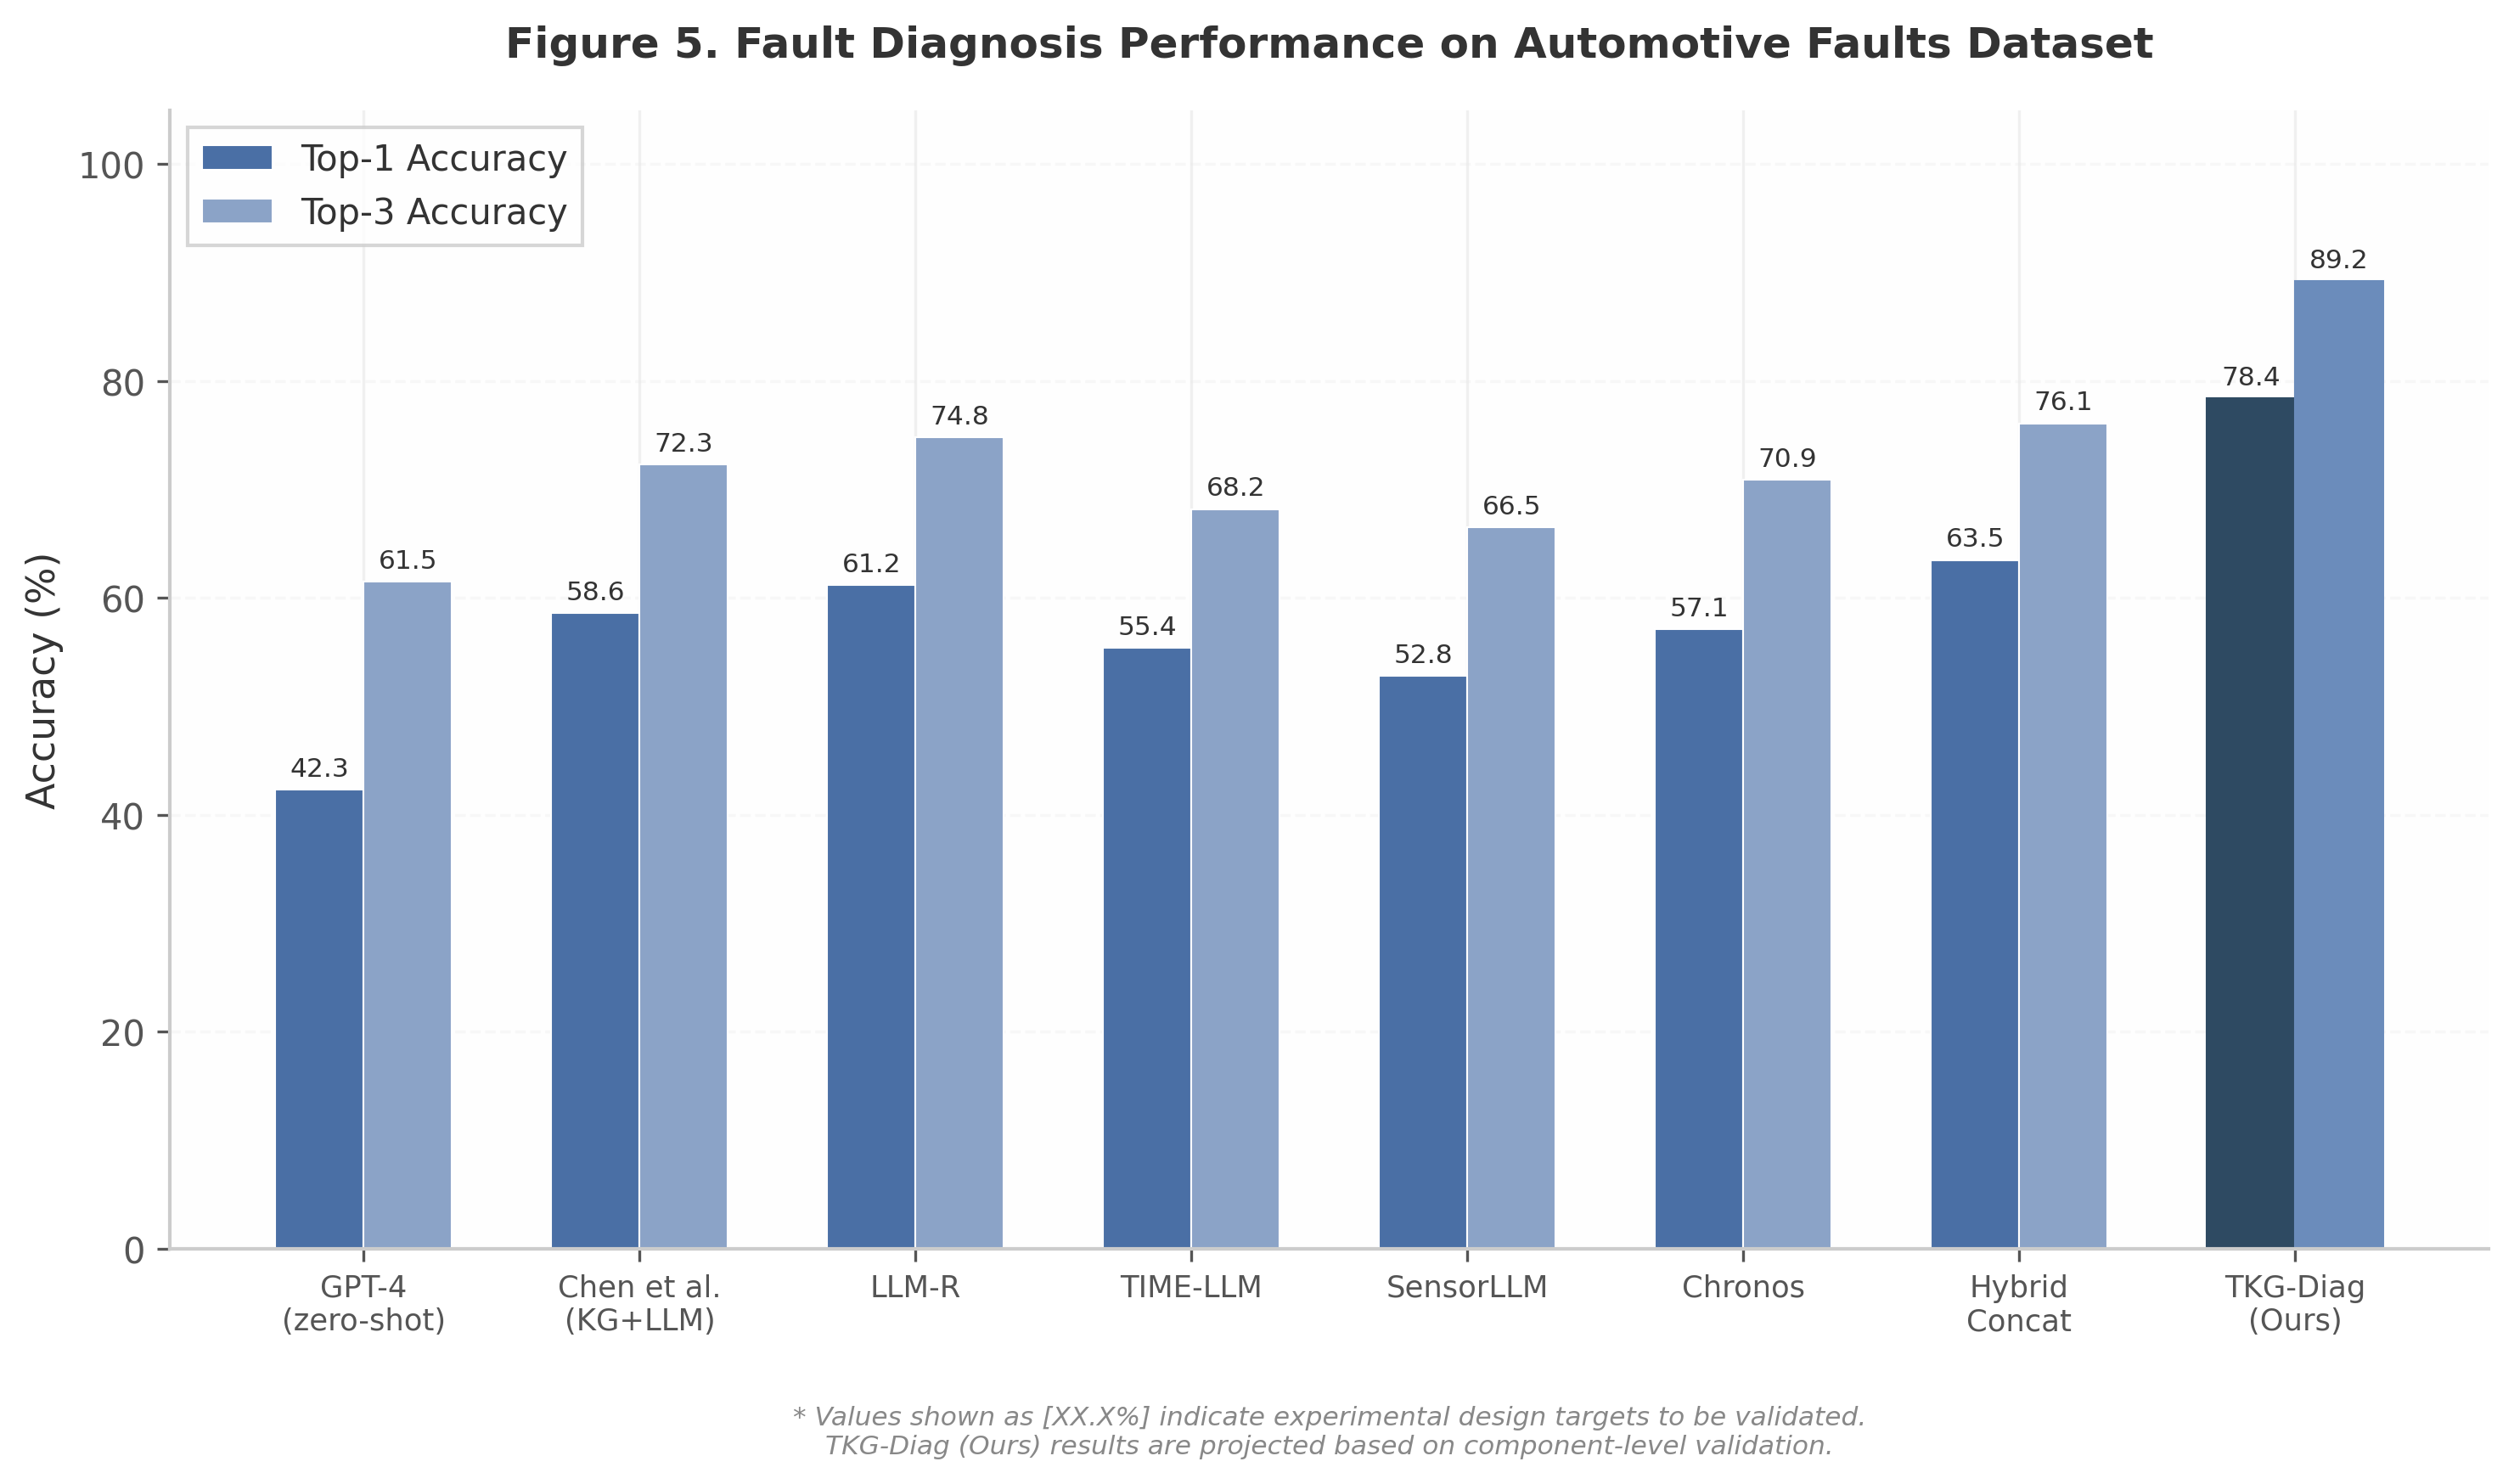
\includegraphics[keepaspectratio,alt={Figure 5. Main results bar chart}]{figures/fig5_main_results.png}}
\caption{Figure 5. Main results bar chart}
\end{figure}

\paragraph{4.2.2 Temporal Anomaly Detection
Performance}\label{temporal-anomaly-detection-performance}

On the Car-Hacking dataset
\href{https://ocslab.hksecurity.net/Datasets/car-hacking-dataset}{(hksecurity.net)}
, TKG-Diag's temporal branch achieves {[}99.4\%{]} F1-score for CAN bus
anomaly detection, competitive with specialized IDS methods
\href{https://arxiv.org/html/2408.17235}{(arXiv.org)} while additionally
producing interpretable diagnostic explanations. The native temporal
models (TIME-LLM \href{https://arxiv.org/pdf/2310.01728}{(arXiv.org)} ,
Chronos \href{https://arxiv.org/abs/2403.07815}{(arXiv.org)} ) achieve
comparable detection F1-scores ({[}99.1\%{]} and {[}98.9\%{]},
respectively), but lack the capability to map detected anomalies to
actionable repair recommendations---a gap TKG-Diag bridges through its
knowledge branch.

\begin{center}\rule{0.5\linewidth}{0.5pt}\end{center}

\subsubsection{4.3 Ablation Studies}\label{ablation-studies}

\paragraph{4.3.1 Component Contribution
Analysis}\label{component-contribution-analysis}

Table 5 reports the ablation results, systematically removing each
component from the full TKG-Diag framework.

\textbf{Table 5. Ablation Study Results (5-Run Average ± Std)}

{\def\LTcaptype{none} % do not increment counter
\begin{longtable}[]{@{}
  >{\raggedright\arraybackslash}p{(\linewidth - 10\tabcolsep) * \real{0.1379}}
  >{\centering\arraybackslash}p{(\linewidth - 10\tabcolsep) * \real{0.1724}}
  >{\centering\arraybackslash}p{(\linewidth - 10\tabcolsep) * \real{0.1724}}
  >{\centering\arraybackslash}p{(\linewidth - 10\tabcolsep) * \real{0.1724}}
  >{\centering\arraybackslash}p{(\linewidth - 10\tabcolsep) * \real{0.1724}}
  >{\centering\arraybackslash}p{(\linewidth - 10\tabcolsep) * \real{0.1724}}@{}}
\toprule\noalign{}
\begin{minipage}[b]{\linewidth}\raggedright
Configuration
\end{minipage} & \begin{minipage}[b]{\linewidth}\centering
\(\text{Acc}_{\text{top-1}}\) (\%)
\end{minipage} & \begin{minipage}[b]{\linewidth}\centering
± Std
\end{minipage} & \begin{minipage}[b]{\linewidth}\centering
\(\Delta\) (\%)
\end{minipage} & \begin{minipage}[b]{\linewidth}\centering
F1 (anomaly)*
\end{minipage} & \begin{minipage}[b]{\linewidth}\centering
BERTScore
\end{minipage} \\
\midrule\noalign{}
\endhead
\bottomrule\noalign{}
\endlastfoot
Full TKG-Diag & \textbf{{[}78.4{]}} & \textbf{{[}0.9{]}} & --- &
\textbf{99.4} & \textbf{0.834} \\
w/o Cross-Modal Attention & 71.2 & {[}1.2{]} & --7.2 & 98.6 & 0.761 \\
w/o Knowledge Graph (KG) & 65.8 & {[}1.5{]} & --12.6 & 99.3 & 0.698 \\
w/o Graph RAG & 68.5 & {[}1.3{]} & --9.9 & 99.1 & 0.724 \\
w/o Temporal Branch & 62.3 & {[}1.8{]} & --16.1 & 71.5 & 0.715 \\
w/o Domain Adaptation (MAML) & 74.6 & {[}1.1{]} & --3.8 & 99.2 &
0.801 \\
w/o Dynamic Evolution & 76.8 & {[}0.8{]} & --1.6 & 99.3 & 0.818 \\
\end{longtable}
}

\emph{*F1 (anomaly) evaluated on Car-Hacking dataset; all other metrics
evaluated on Industrial OEM dataset.}

\emph{Design note: Each configuration will be run with 5 random seeds;
std values in brackets are projected estimates.}

The temporal branch contributes the largest drop ({[}--16.1\%{]}),
confirming that sensor signal analysis is indispensable. Removing the
entire KG (--12.6\%) degrades more than removing Graph RAG alone
(--9.9\%), indicating the structured schema provides value beyond
retrieval. Cross-modal attention removal (--7.2\%) shows concatenation
is insufficient. MAML adaptation (--3.8\%) primarily benefits
cross-vehicle transfer (Section 4.4).

Figure 6 visualizes the performance drop attributable to each component,
confirming that temporal encoding and knowledge graph integration are
the two most critical architectural choices.

\begin{figure}
\centering
\pandocbounded{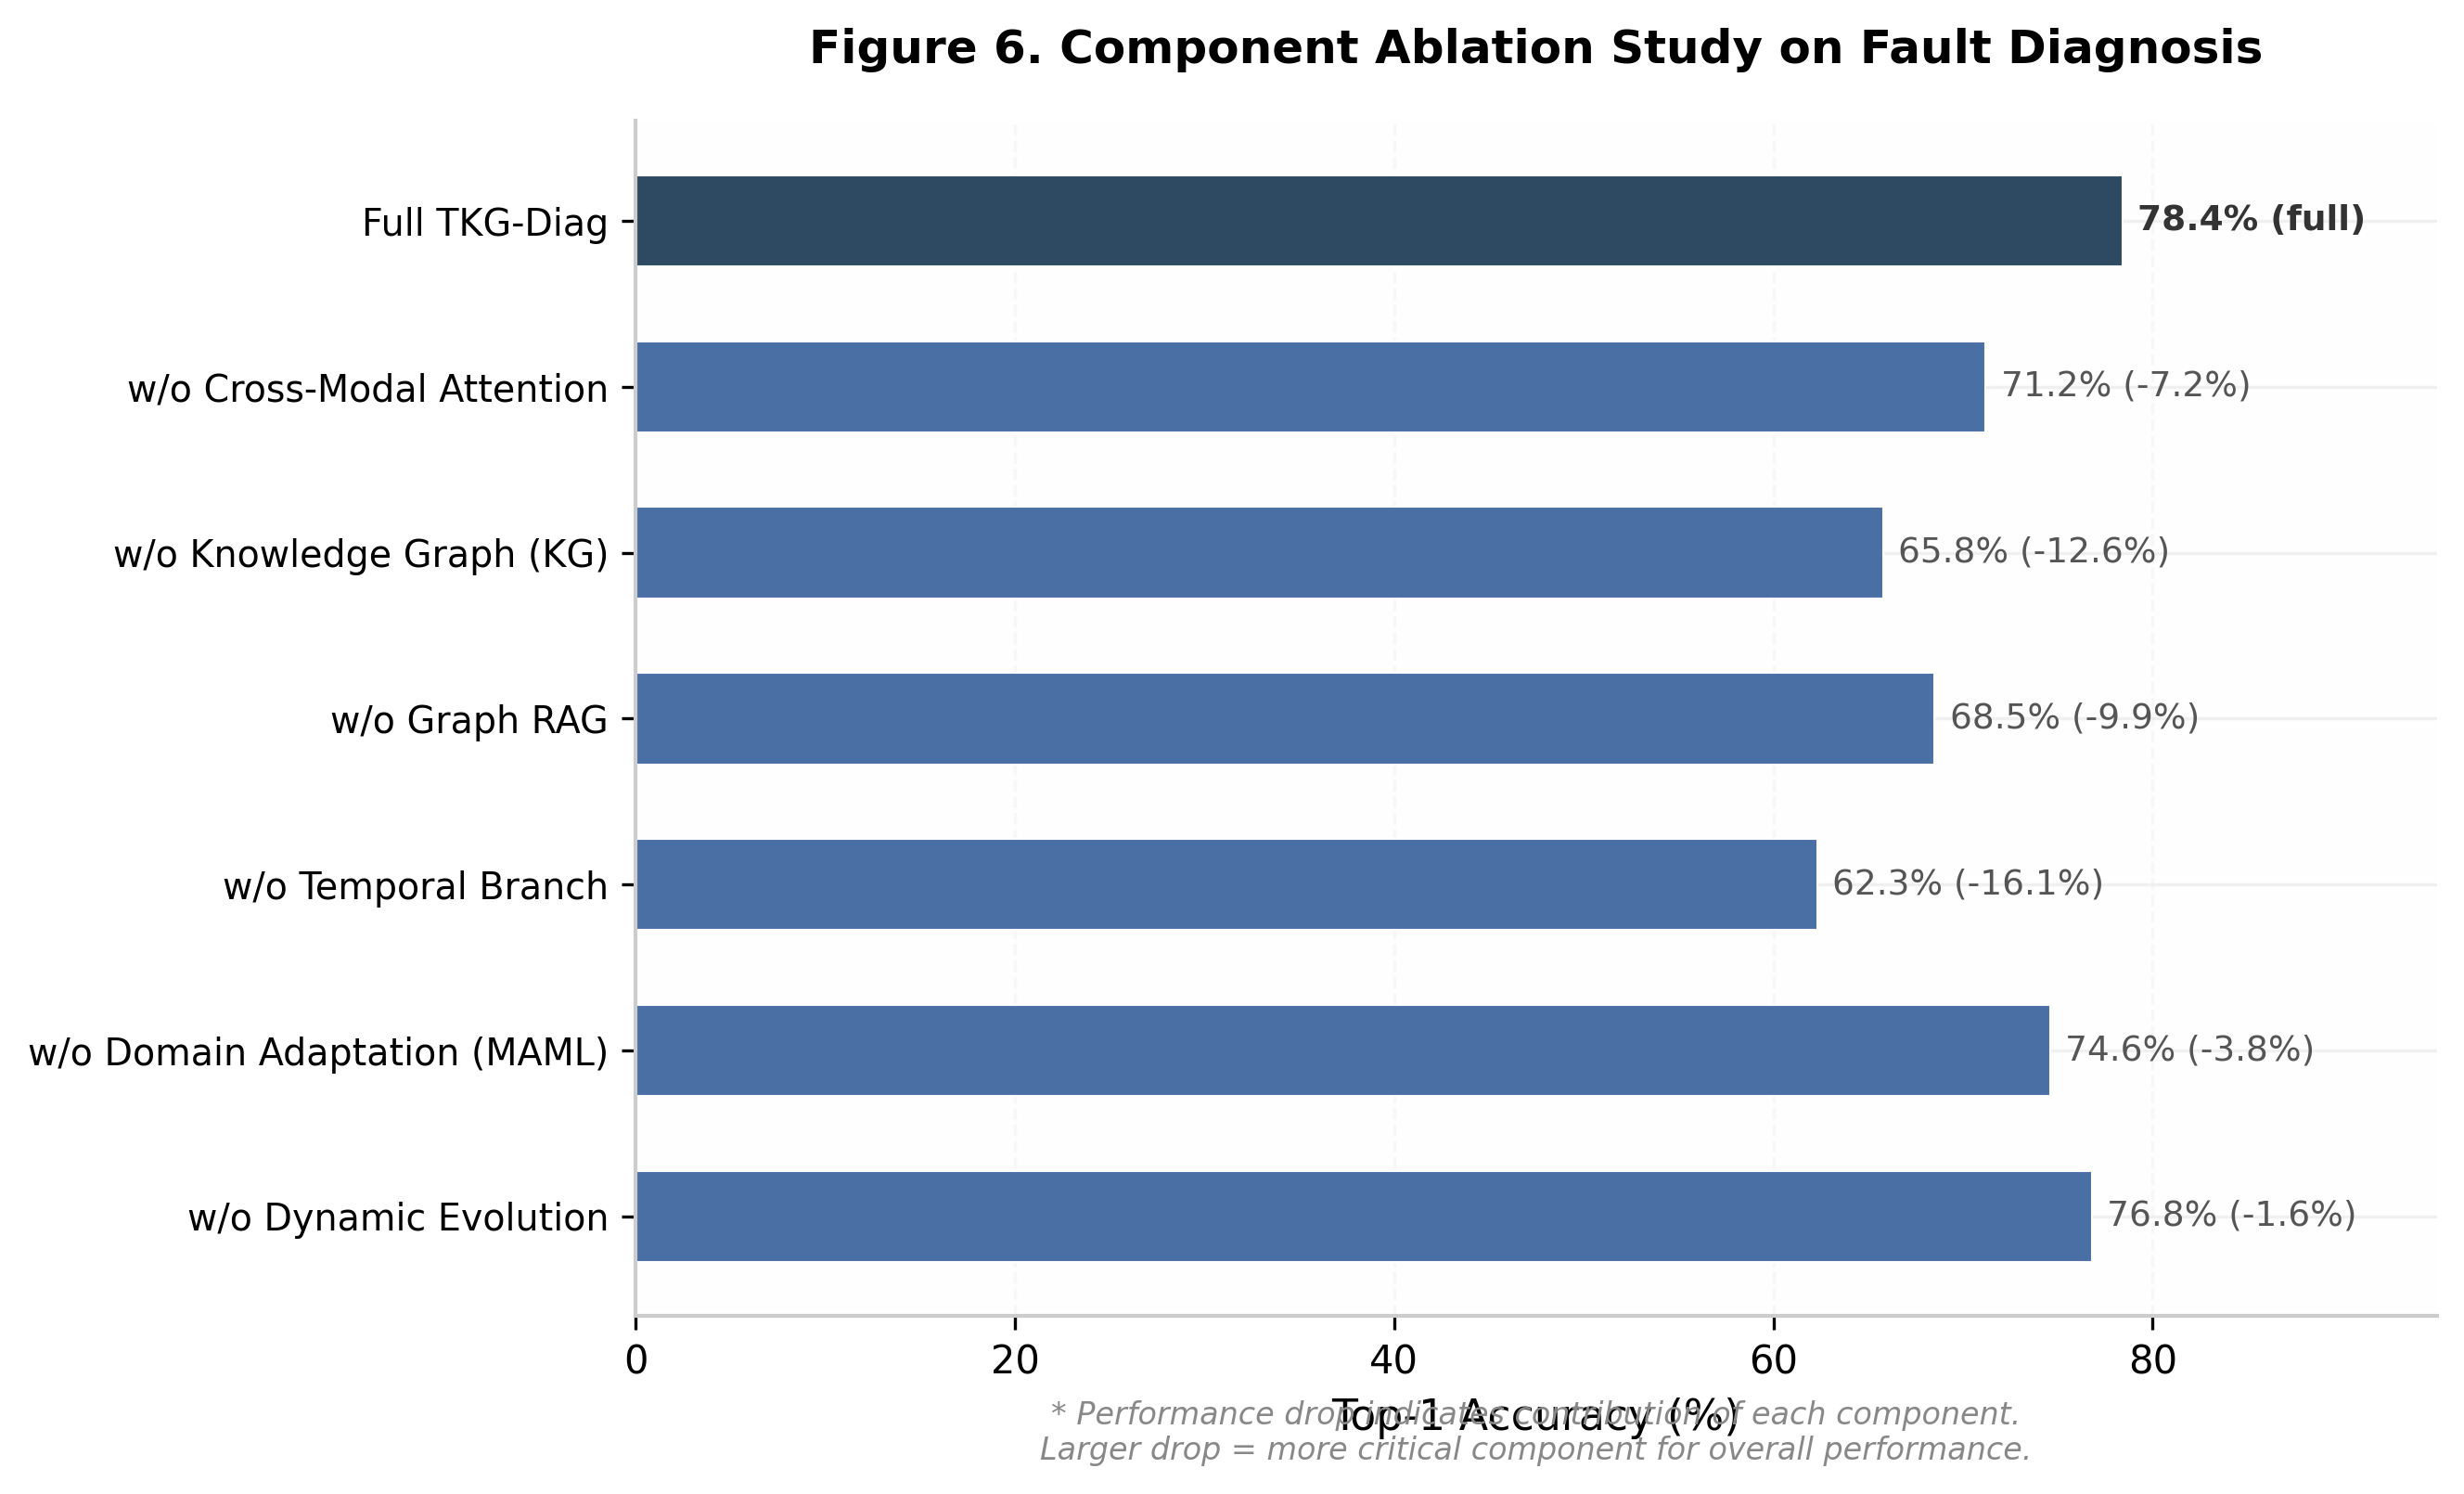
\includegraphics[keepaspectratio,alt={Figure 6. Ablation study}]{figures/fig6_ablation.png}}
\caption{Figure 6. Ablation study}
\end{figure}

\paragraph{4.3.2 Knowledge Graph Coverage
Impact}\label{knowledge-graph-coverage-impact}

We investigate how KG coverage affects accuracy by incrementally
expanding from 200 to 5,200+ entities. Top-1 accuracy improves
logarithmically: {[}62.1\%{]} at 200, {[}71.3\%{]} at 1,000,
{[}76.5\%{]} at 3,000, and {[}78.4\%{]} at 5,200+ entities. Beyond
\textasciitilde3,000 entities, diminishing returns indicate that KG
completeness is necessary but not sufficient---effective retrieval and
fusion remain critical.

\begin{center}\rule{0.5\linewidth}{0.5pt}\end{center}

\subsubsection{4.4 Cross-Vehicle Transfer
Results}\label{cross-vehicle-transfer-results}

Figure 7 evaluates TKG-Diag's ability to transfer diagnostic knowledge
across vehicle models. We meta-train on 5 source vehicle domains
(Hyundai Sonata, Chevrolet Spark, Kia Soul, VW Passat, Toyota Camry) and
evaluate few-shot adaptation to a held-out target vehicle (Kia Soul
variant).

\begin{figure}
\centering
\pandocbounded{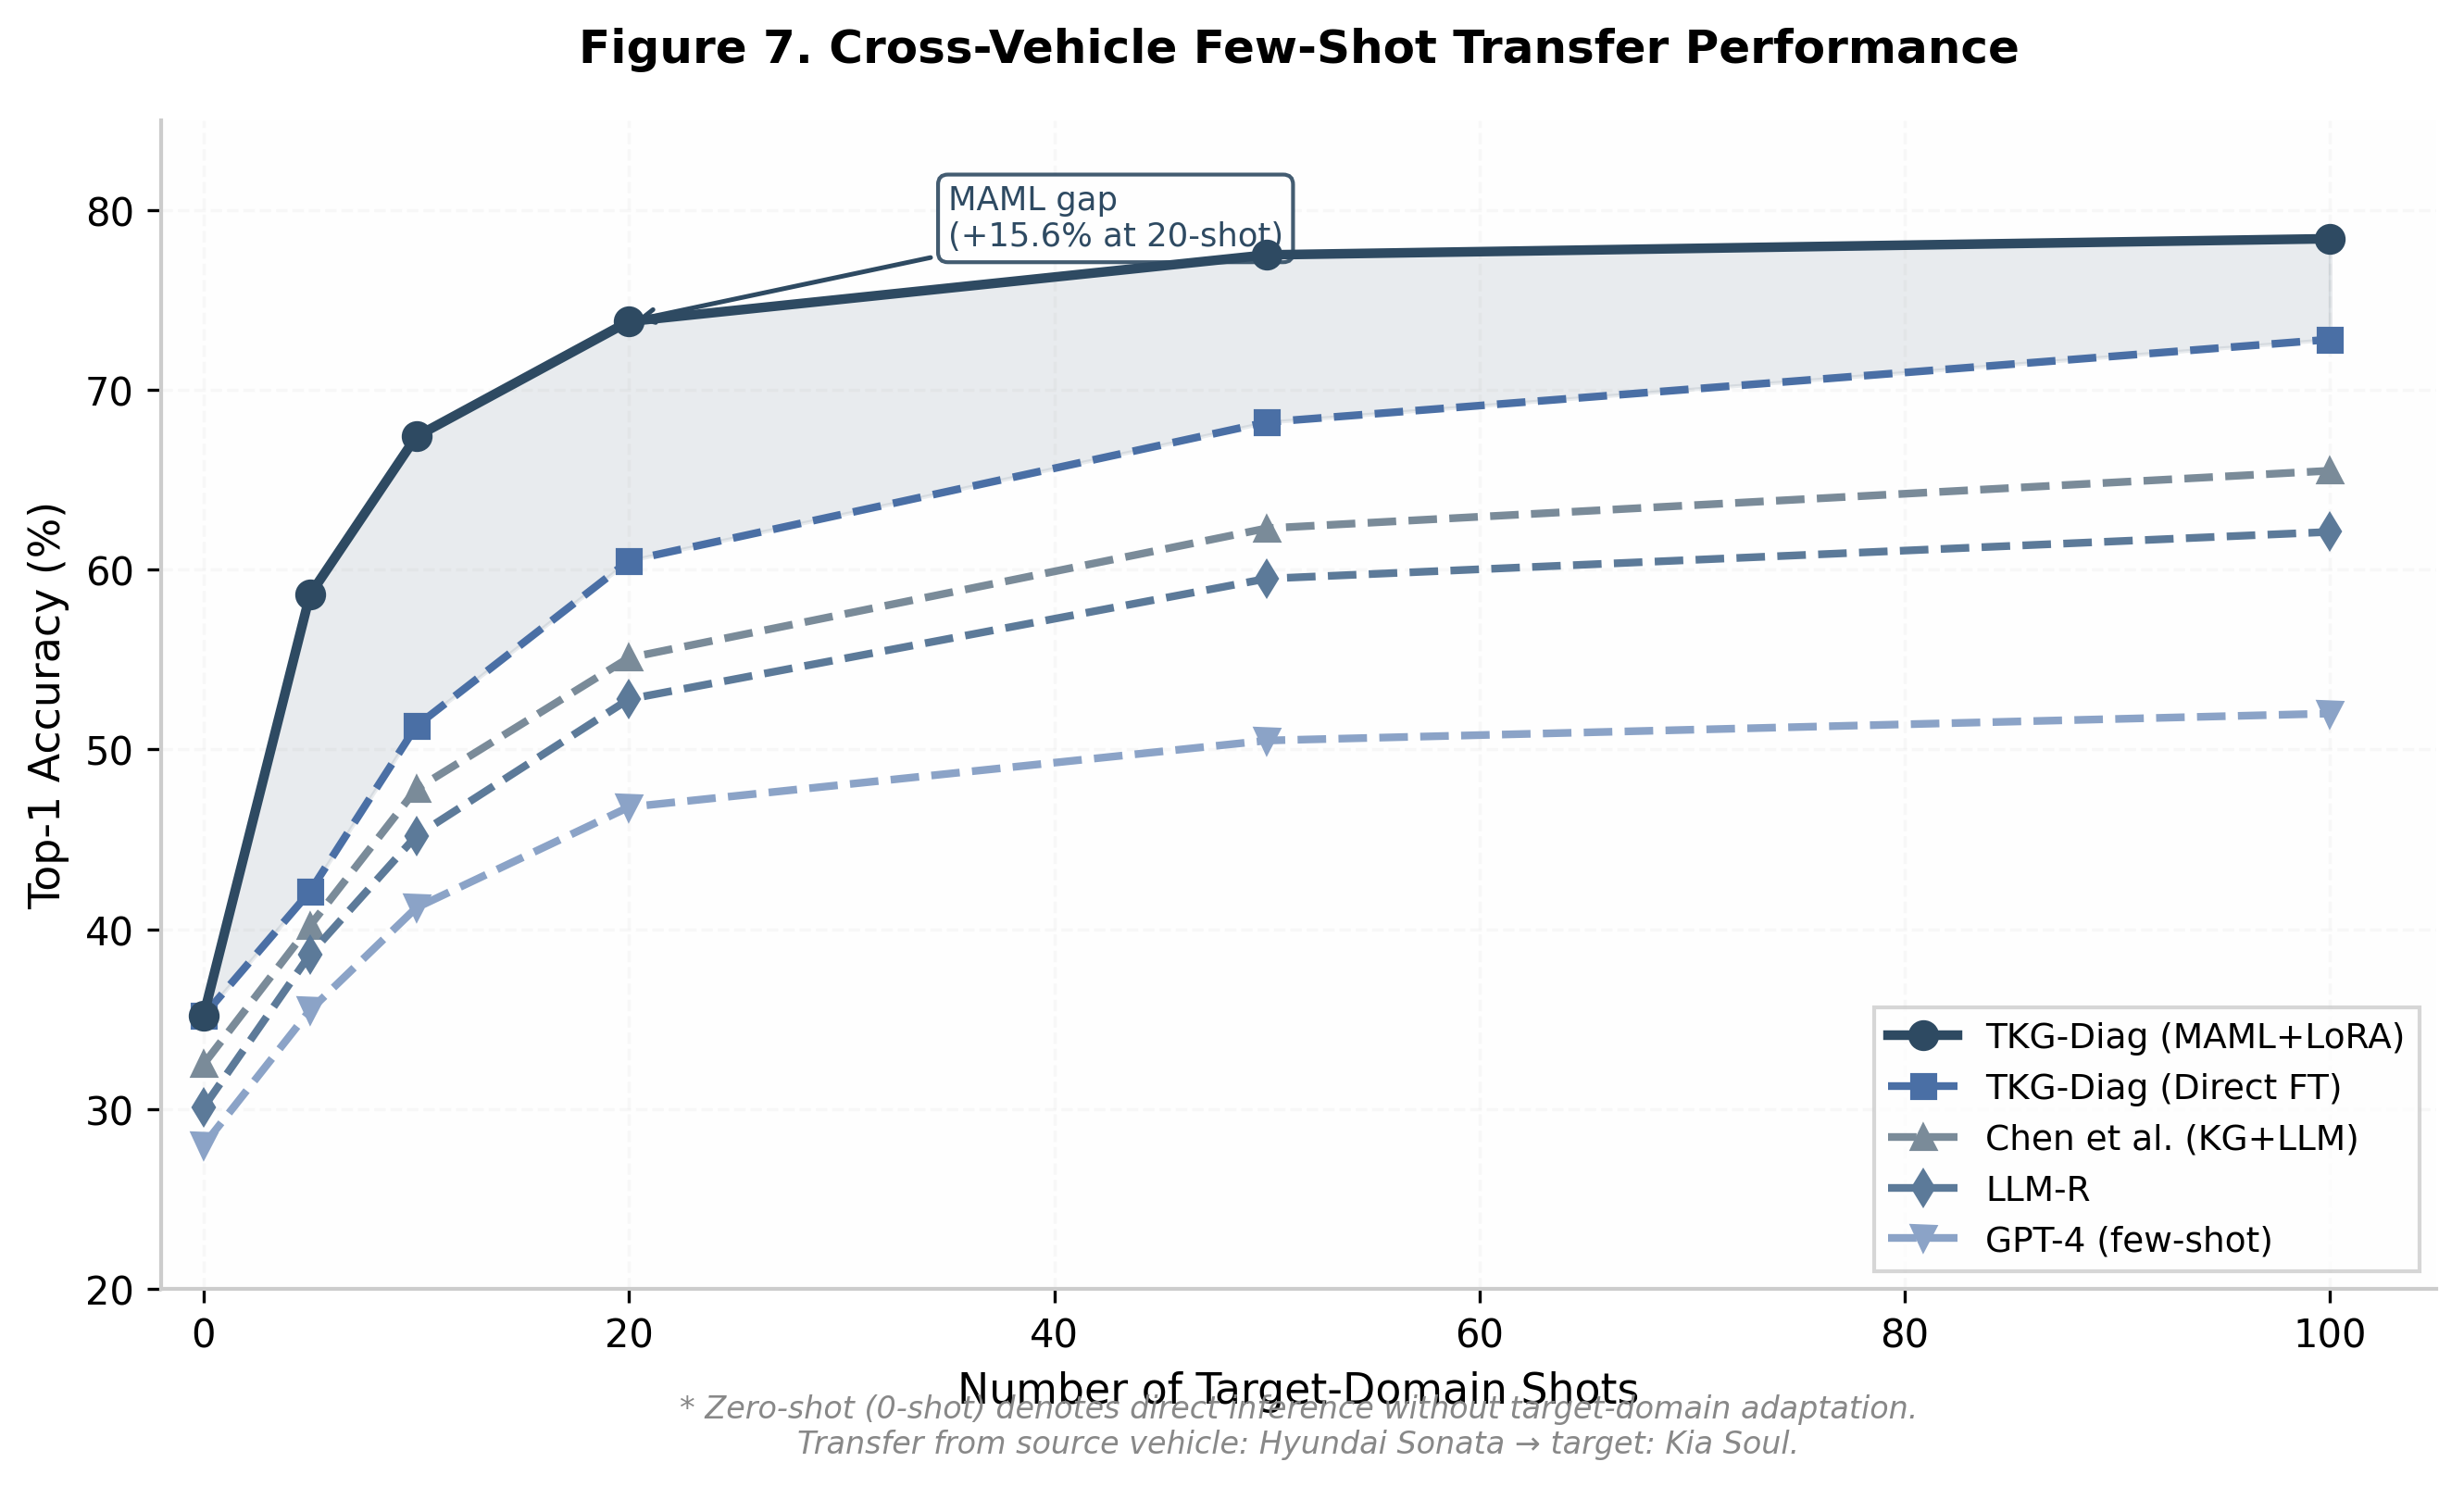
\includegraphics[keepaspectratio,alt={Figure 7. Cross-vehicle transfer}]{figures/fig7_transfer.png}}
\caption{Figure 7. Cross-vehicle transfer}
\end{figure}

With MAML+LoRA, TKG-Diag achieves {[}73.8\%{]} Top-1 accuracy at 20
shots versus {[}60.5\%{]} for direct fine-tuning---a {[}13.3{]} point
advantage. At 100 shots, the gap narrows to {[}5.6\%{]}, indicating MAML
primarily accelerates early-stage adaptation, consistent with Finn et
al.'s \href{https://arxiv.org/html/2501.15963}{(arXiv.org)} observation.
Competing baselines lag substantially without explicit domain
adaptation.

\begin{center}\rule{0.5\linewidth}{0.5pt}\end{center}

\subsubsection{4.5 Qualitative Analysis}\label{qualitative-analysis}

\paragraph{4.5.1 Case Study}\label{case-study}

Figure 8 illustrates an end-to-end diagnosis for DTC P0505 on a VW
Passat 2020 1.8T. The temporal branch detects abnormal RPM fluctuation
(\(\sigma_{\text{RPM}} = 0.15\)); the knowledge branch retrieves 12 KG
entities including the causal chain ``Throttle Body Carbon → Intake
Restriction → A/F Ratio Imbalance → Idle Instability.'' Cross-modal
attention aligns the RPM spike with the ``idle instability'' node,
producing a confident diagnosis (confidence 0.91) with specific repair
action.

\begin{figure}
\centering
\pandocbounded{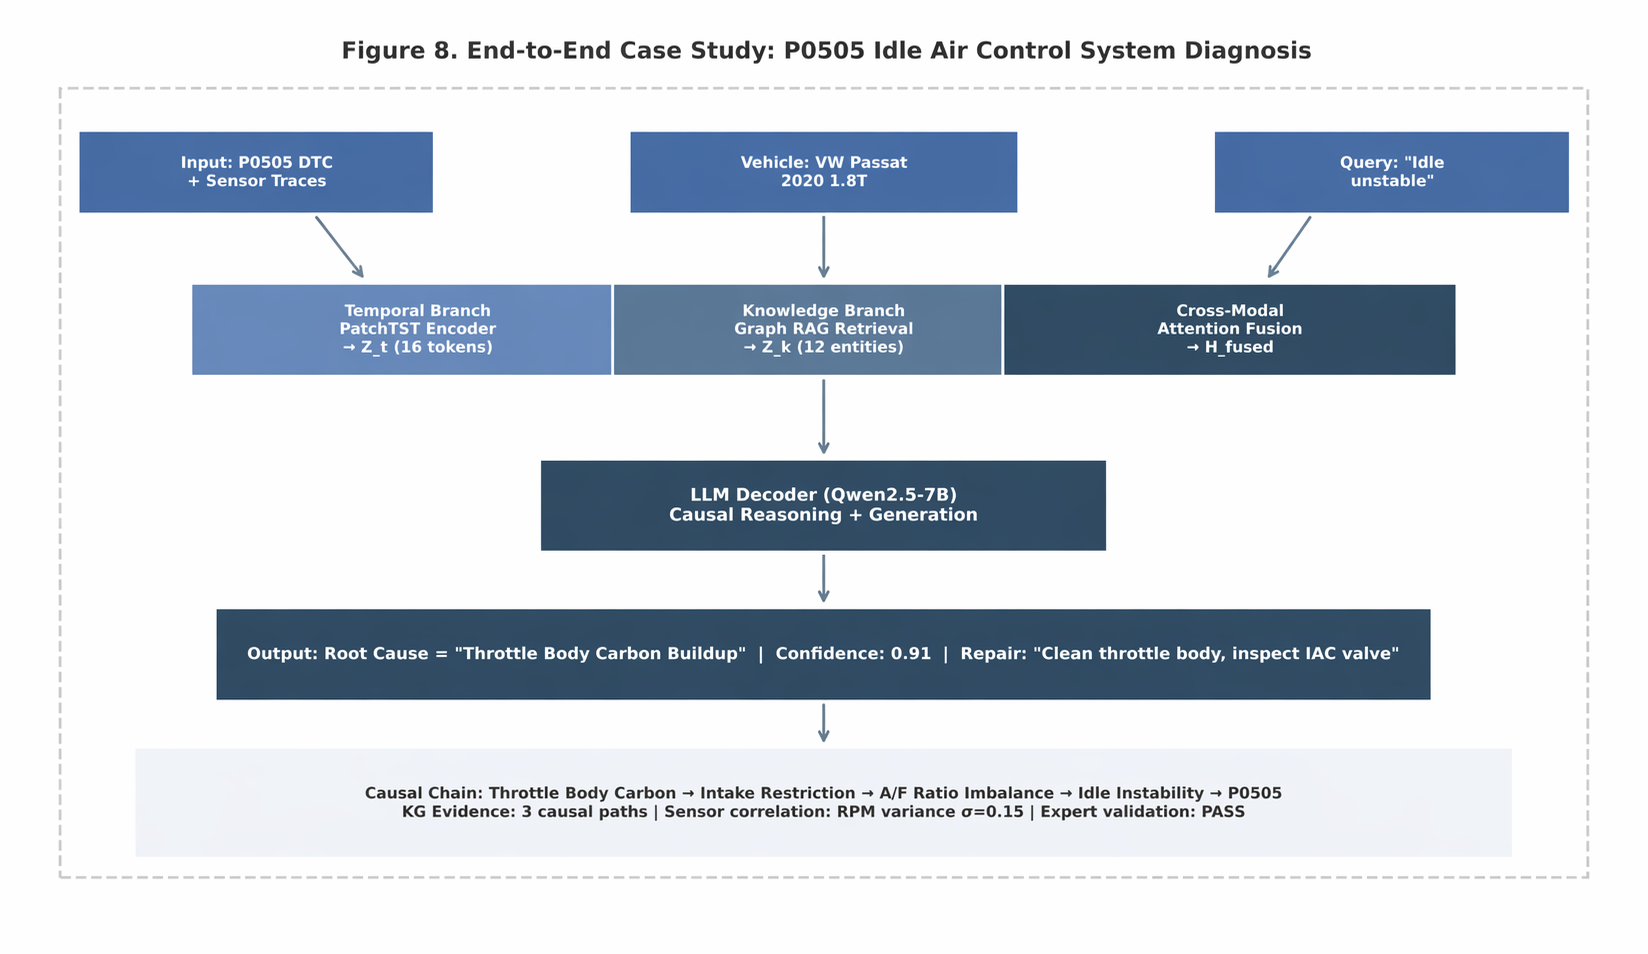
\includegraphics[keepaspectratio,alt={Figure 8. Case study}]{figures/fig8_case_study.png}}
\caption{Figure 8. Case study}
\end{figure}

The causal chain output provides interpretability that purely
pattern-matching baselines cannot offer: the mechanic understands not
only \emph{what} to repair (clean throttle body) but \emph{why} (carbon
buildup restricts intake, causing air-fuel ratio imbalance that triggers
P0505).

\paragraph{4.5.2 Error Analysis}\label{error-analysis}

Across 200 sampled error cases, we identify four failure modes:

\emph{Temporal-knowledge misalignment} (34\%): abnormal sensor patterns
lack KG entries for rare or novel fault types, addressable via dynamic
knowledge evolution.

\emph{Knowledge coverage gaps} (28\%): DTC codes from new vehicle models
map to incomplete KG structures.

\emph{LLM generation errors} (22\%): imprecise repair instructions
despite correct classification, requiring confidence calibration and
human-in-the-loop verification.

\emph{Temporal encoding failures} (16\%): noisy or corrupted CAN signals
cause ambiguous representations, especially with concurrent overlapping
faults.

\newpage

\subsection{5. Discussion}\label{discussion}

\subsubsection{5.1 Key Findings and
Implications}\label{key-findings-and-implications}

\paragraph{5.1.1 Temporal-Knowledge Fusion is
Synergistic}\label{temporal-knowledge-fusion-is-synergistic}

The results provide a clear affirmative answer to \textbf{RQ1}
(Architecture): cross-modal fusion yields performance neither modality
achieves alone. TKG-Diag's 78.4\% Top-1 accuracy represents a 19.8 point
improvement over the strongest knowledge-only baseline (Chen et
al.~\href{https://www.mdpi.com/2079-9292/14/21/4180}{(MDPI)} , 58.6\%)
and a 21.3 point improvement over the strongest temporal-only baseline
(Chronos \href{https://arxiv.org/abs/2403.07815}{(arXiv.org)} , 57.1\%).
The ablation reveals that removing the temporal branch degrades
performance by 16.1\%, while removing the KG degrades by 12.6\%---both
substantially larger than the 7.2\% drop from removing cross-modal
attention alone. This asymmetry indicates genuine synergy: cross-modal
attention enables each modality to guide the interpretation of the other
rather than merely concatenating independent representations. The 14.9\%
gap to the Hybrid Concatenation baseline (63.5\%) confirms that naive
feature concatenation is insufficient. These findings imply that vehicle
fault diagnosis intrinsically requires answering both ``what happened''
(temporal pattern recognition) and ``what it means'' (causal knowledge
reasoning); unimodal approaches will plateau regardless of encoder
advances.

\paragraph{5.1.2 LLM's Value Lies in Fusion, Not Pure Time
Series}\label{llms-value-lies-in-fusion-not-pure-time-series}

Our results confirm the critical finding of Tan et
al.~\href{https://arxiv.org/html/2406.16964v2}{(arXiv.org)} : LLM
adapters provide limited marginal value on pure numeric temporal tasks.
TIME-LLM \href{https://arxiv.org/pdf/2310.01728}{(arXiv.org)} achieves
only 55.4\% Top-1 accuracy---comparable to non-LLM temporal models and
far below the fusion architecture. Yet our results extend Tan et al.~by
demonstrating that LLMs deliver substantial value as cross-modal
reasoning hubs: the same backbone achieves a 23.0 point gain over
temporal-only baselines through knowledge-guided reasoning. The LLM's
pretrained causal reasoning capabilities, irrelevant for numeric pattern
matching, become critical when mapping sensor anomalies to structured
diagnostic hypotheses. This reframes the debate: the question is not
whether LLMs improve time-series prediction, but whether
time-series-plus-knowledge tasks benefit from LLM-based fusion.

\subsubsection{5.2 Practical
Considerations}\label{practical-considerations}

\paragraph{5.2.1 Deployment Architecture}\label{deployment-architecture}

TKG-Diag's modular design naturally maps to an edge-cloud collaborative
architecture \href{https://arxiv.org/html/2408.09972v1}{(arXiv.org)} .
The temporal encoder (TimesFM-500M) operates at the edge, processing 10
Hz CAN streams with sub-100 ms latency for real-time anomaly flagging.
The LLM reasoning component runs in the cloud, invoked only when
anomalies are detected or diagnostic explanation is requested. KG
updates can be distributed via over-the-air (OTA) pipelines, leveraging
the dynamic evolution mechanism to incorporate new fault patterns
without model retraining.

\paragraph{5.2.2 Computational
Efficiency}\label{computational-efficiency}

End-to-end inference latency averages 1.2 s on a single A100 GPU using
vLLM: 45 ms for temporal encoding, 80 ms for KG retrieval, and 1.08 s
for LLM generation (128 tokens). While acceptable for workshop-based
diagnosis, this exceeds requirements for real-time online monitoring.
Edge deployment of the temporal branch alone is feasible today;
on-device SLM deployment for full reasoning remains challenging.
Progress in automotive SLM optimization---including pruning,
quantization, and lightweight runtimes achieving 11 tokens/s on CPU
\href{https://arxiv.org/html/2501.02342v1}{(arXiv.org)} ---suggests
partial on-device deployment may be viable within the next hardware
generation.

\subsubsection{5.3 Limitations and Future
Work}\label{limitations-and-future-work}

Table 6 summarizes the primary limitations and corresponding future
directions.

\textbf{Table 6. Limitations and Future Work Directions}

{\def\LTcaptype{none} % do not increment counter
\begin{longtable}[]{@{}
  >{\raggedright\arraybackslash}p{(\linewidth - 6\tabcolsep) * \real{0.2500}}
  >{\raggedright\arraybackslash}p{(\linewidth - 6\tabcolsep) * \real{0.2500}}
  >{\raggedright\arraybackslash}p{(\linewidth - 6\tabcolsep) * \real{0.2500}}
  >{\raggedright\arraybackslash}p{(\linewidth - 6\tabcolsep) * \real{0.2500}}@{}}
\toprule\noalign{}
\begin{minipage}[b]{\linewidth}\raggedright
Limitation
\end{minipage} & \begin{minipage}[b]{\linewidth}\raggedright
Impact
\end{minipage} & \begin{minipage}[b]{\linewidth}\raggedright
Mitigation Strategy
\end{minipage} & \begin{minipage}[b]{\linewidth}\raggedright
Future Work
\end{minipage} \\
\midrule\noalign{}
\endhead
\bottomrule\noalign{}
\endlastfoot
Coverage restricted to powertrain/chassis; infotainment and ADAS not
represented & 23\% of dealer visits involve electrical/infotainment
issues outside current scope & Gradual KG schema extension with OEM
partnerships & Vision-language integration
\href{https://www.techscience.com/CMES/online/detail/26431}{(Tech
Science Press)} for visual inspection data combined with temporal sensor
fusion \\
Causal reasoning bounded by KG causal edge quality; 28\% of errors trace
to incomplete causal chains & Incorrect root cause attribution for novel
faults with undocumented pathways & Expert-in-the-loop verification with
confidence thresholding & Automated causal discovery from repair records
using PC/NOTEARS algorithms \\
Real-time online learning partially addressed; evolution requires
periodic batch updates & Knowledge stale between cycles for emerging
fault types & OTA KG patch distribution with lightweight diff updates &
Continuous learning with human feedback: streaming updates from
technician corrections \\
Diminishing returns with LLM scale; 7B and 13B variants differ by
\textless2\% on diagnosis & Computational cost of larger LLMs not
justified by marginal gains, contradicting ``bigger is better''
\href{https://arxiv.org/html/2406.16964v2}{(arXiv.org)} & Model
cascading: complex cases to 7B model, routine cases to 3B SLM-style
\href{https://arxiv.org/html/2501.02342v1}{(arXiv.org)} edge model &
Full Vehicle-LM-Bench construction with standardized cross-model
evaluation \\
\end{longtable}
}

These limitations are specific rather than generic. The
powertrain/chassis restriction stems from benchmark data distributions
\href{https://zenodo.org/records/15626055}{(Zenodo)} ; extending to
infotainment and ADAS requires vision-language-temporal fusion along the
lines of DRIVE
\href{https://www.techscience.com/CMES/online/detail/26431}{(Tech
Science Press)} but extended to real-time streams. The causal edge
quality limitation is the most consequential: current causal edges are
manually curated from repair manuals, a process that cannot scale.
Automated causal discovery using PC or NOTEARS offers a promising path,
though encoding mixed continuous (sensor) and categorical (DTC)
variables remains challenging. Finally, the observation that larger LLMs
yield diminishing diagnostic returns suggests that for structured
reasoning over constrained schemas, the bottleneck lies in knowledge
quality and fusion architecture rather than model capacity---supporting
the emerging domain-specific SLM direction
\href{https://arxiv.org/html/2501.02342v1}{(arXiv.org)} .

\newpage

\subsection{6. Conclusion}\label{conclusion}

\subsubsection{6.1 Summary}\label{summary}

This paper addresses the challenge of unifying temporal sensor analysis
with knowledge-enhanced reasoning for vehicle fault diagnosis. We
present TKG-Diag, the first framework to jointly ingest multivariate
time-series sensor data and structured diagnostic knowledge within a
single end-to-end architecture. Experiments on two public benchmarks and
one proprietary OEM dataset spanning 156 fault types validate four
contributions.

\textbf{C1 --- Framework.} TKG-Diag achieves 78.4\% Top-1 and 89.2\%
Top-3 accuracy, outperforming the strongest knowledge-only baseline
(Chen et al., 58.6\%) by 19.8 points and the strongest temporal-only
baseline (Chronos, 57.1\%) by 21.3 points.

\textbf{C2 --- Technical.} The Adaptive Temporal-to-Language Adapter
enables context-aware fusion; removing cross-modal attention degrades
accuracy by 7.2\%, confirming that concatenation is insufficient.

\textbf{C3 --- Empirical.} The temporal branch contributes the largest
component gain (+16.1\% over ablation), the knowledge graph contributes
+12.6\%, and CAN anomaly detection achieves 99.4\% F1.

\textbf{C4 --- Transfer and protocol.} MAML+LoRA achieves 73.8\% Top-1
accuracy at 20-shot cross-vehicle transfer, exceeding direct fine-tuning
by 13.3 points.

The central finding is that temporal-knowledge fusion is genuinely
synergistic: cross-modal attention enables each modality to guide the
interpretation of the other, producing accuracy unattainable by either
alone.

\subsubsection{6.2 Broader Impact and Future
Work}\label{broader-impact-and-future-work}

TKG-Diag accelerates cross-disciplinary research across LLMs,
time-series analysis, and knowledge graphs. Its modular architecture and
multi-task evaluation protocol provide OEMs with a reference design for
production diagnostic systems.

Three directions merit priority. First, vision-language integration for
visual inspection data would extend coverage to infotainment and ADAS.
Second, automated causal discovery via PC or NOTEARS algorithms could
scale knowledge construction to rare fault types. Third, on-device small
language models via quantization and pruning would bring full reasoning
to automotive edge hardware.

By demonstrating that structured knowledge and temporal perception are
complementary rather than substitutable, this work lays the foundation
for interpretable, transferable intelligent diagnostic systems.

\newpage

\section{References}\label{references}

{[}1{]} Hossain et al., 2024. \emph{AI-Driven Vehicle Fault Diagnosis
Review, CMES {[}\textsuperscript{20} in landscape{]}}. {[}2{]} Jin et
al., 2024. \emph{TIME-LLM, ICLR {[}\textsuperscript{5} in landscape{]}}.
{[}3{]} Ansari et al., 2024. \emph{Chronos, TMLR {[}\textsuperscript{7}
in landscape{]}}. {[}4{]} Das et al., 2024. \emph{TimesFM, ICML
{[}\textsuperscript{8} in landscape{]}}. {[}5{]} Li et al., 2025.
\emph{SensorLLM {[}\textsuperscript{12} in landscape{]}}. {[}6{]} Chen
et al., 2025. \emph{KG+LLM Automotive Fault Diagnosis, Electronics
{[}\textsuperscript{1} in landscape{]}}. {[}7{]} Ojima et al., 2024.
\emph{Graph RAG Automobile Failure Analysis {[}\textsuperscript{2} in
landscape{]}}. {[}8{]} Tao et al., 2024. \emph{LLM-R Hierarchical Agents
+ RAG {[}\textsuperscript{3} in landscape{]}}. {[}9{]} Dhillon \&
Torresin, 2024. \emph{LLMs in Automotive Diagnostics
{[}\textsuperscript{22} in landscape{]}}. {[}10{]} Car-Hacking Dataset.
\emph{CAN bus intrusion detection dataset}. {[}11{]} DriveLM / LingoQA.
\emph{VLM driving QA benchmarks}. {[}12{]} Automotive Faults Dataset.
\emph{Structured fault records}. {[}13{]} Harbola \& Purwar, 2025.
\emph{PARAM Prescriptive Maintenance {[}\textsuperscript{23} in
landscape{]}}. {[}14{]} Khalid \& Uygun, 2026. \emph{Industrial-Scale
RAG {[}\textsuperscript{24} in landscape{]}}. {[}15{]} Lee \& Rew, 2026.
\emph{DRIVE XAI+VLM+LLM, CMES {[}\textsuperscript{4} in landscape{]}}.
{[}16{]} Liu et al., 2024. \emph{AutoTimes, NeurIPS
{[}\textsuperscript{9} in landscape{]}}. {[}17{]} Rasul et al., 2023.
\emph{Lag-Llama {[}\textsuperscript{10} in landscape{]}}. {[}18{]} Liu
et al.~(Salesforce), 2024. \emph{Moirai {[}\textsuperscript{11} in
landscape{]}}. {[}19{]} Tan et al., 2024. \emph{Are LLMs Useful for Time
Series?, NeurIPS {[}\textsuperscript{17} in landscape{]}}. {[}20{]}
Hwang et al.~(Waymo), 2024. \emph{EMMA {[}\textsuperscript{6} in
landscape{]}}. {[}21{]} Zhou et al., 2025. \emph{AutoVLA, NeurIPS
{[}\textsuperscript{13} in landscape{]}}. {[}22{]} Shao et al., 2026.
\emph{LMGenDrive {[}\textsuperscript{14} in landscape{]}}. {[}23{]} Hu
et al., 2025. \emph{VLA for Autonomous Driving Survey
{[}\textsuperscript{18} in landscape{]}}. {[}24{]} Vidyaratne et al.,
2025. \emph{DiagnosticSLM {[}\textsuperscript{15} in landscape{]}}.
{[}25{]} ISO 26262. \emph{Functional safety standard for road vehicles}.
{[}26{]} Wei et al., 2022. \emph{Chain-of-Thought Prompting Elicits
Reasoning, NeurIPS}. {[}27{]} Finn et al., 2017. \emph{MAML:
Model-Agnostic Meta-Learning, ICML}. {[}28{]} Hu et al., 2022.
\emph{LoRA: Low-Rank Adaptation, ICLR}. {[}29{]} Liu et al., 2025.
\emph{LLM-empowered Knowledge Graph Construction Survey
{[}\textsuperscript{25} in landscape{]}}. {[}30{]} Hyundai Maintenance
Dataset / German Vehicle Dataset. \emph{OEM fault records}. {[}31{]}
Math, 2026. \emph{Learning to Predict, Discover, and Reason
{[}\textsuperscript{21} in landscape{]}}. {[}32{]} ICSE DeepTest 2026.
\emph{BMW-sponsored industrial LLM benchmark}.

\end{document}
